% SPDX-License-Identifier: CC-BY-4.0
\documentclass[10pt,twocolumn]{article}

\usepackage[a4paper,margin=0.85in]{geometry}
\setlength{\columnsep}{0.33in}
\usepackage{times}
\usepackage{amsmath}
\usepackage{microtype}
\usepackage[utf8]{inputenc}
\usepackage[T1]{fontenc}
\usepackage{graphicx}
\usepackage{xcolor}
\usepackage{booktabs}
\usepackage{multirow}
\usepackage{listings}
\usepackage{url}
\usepackage[hidelinks]{hyperref}
\usepackage{enumitem}
\usepackage{authblk}
\usepackage{abstract}
\usepackage{titlesec}
\usepackage{caption}
\usepackage{subcaption}

\titleformat{\section}{\large\bfseries}{\thesection.}{0.5em}{}
\titleformat{\subsection}{\normalsize\bfseries}{\thesubsection}{0.5em}{}

\setlist{nosep, leftmargin=*}

\lstset{
  basicstyle=\ttfamily\footnotesize,
  breaklines=true,
  columns=fullflexible,
  frame=single,
  showstringspaces=false,
  keepspaces=true,
}

\renewcommand{\abstractname}{\vspace{-1em}}

\title{\textbf{OpenURMA: A Clean-Room Open Implementation of \\
the Unified Bus Protocol}}

\author[1]{Bojie Li}
\affil[1]{Pine AI \\ \texttt{bojieli@gmail.com}}

\date{}

\begin{document}

\twocolumn[
  \begin{@twocolumnfalse}
    \maketitle
    \vspace{-2em}
    \begin{abstract}
      \noindent
      Modern datacenter RDMA is bottlenecked at the network interface,
      not at the wire. At the scale of AI-training collectives and HPC
      all-to-alls, a NIC running RoCE or InfiniBand must hold
      per-connection state for every (application, remote-endpoint)
      pair --- hundreds of megabytes of context at 1024-application
      fanout --- and pays a four-traversal PCIe round trip on the
      smallest 64-byte operation, inflating end-to-end latency by an
      order of magnitude beyond the wire delay. Both costs are
      structural consequences of the Queue-Pair-over-PCIe abstraction
      that commodity RDMA inherits from InfiniBand.

      Huawei's \emph{Unified Bus} (UB) is a public 2025 specification
      that removes both costs by changing the abstraction. Its transport
      protocol decouples per-application endpoint state from per-host
      reliable-transport state, so connection context grows additively
      rather than multiplicatively; it exposes ordering as an opt-in
      surface so applications pay gating only when they need it; and
      it reaches remote memory through a CPU's native load/store
      instructions to a controller on the on-chip bus rather than
      through verbs to a PCIe-attached device. The protocol ships in
      Huawei's Ascend~950 silicon, which is closed.

      \emph{OpenURMA} is the first clean-room open implementation of
      the Unified Bus protocol's transport and transaction layers,
      written from the public specification. We realise it at three
      modeling tiers --- synthesisable RTL on Alveo~U50, a cycle-level
      two-node SystemC simulator that accounts for both endpoints of
      the wire, and a gem5 full-system scaffold in which two ARM CPUs
      run real user binaries against the SystemC NIC --- with a matched
      OpenRoCE (RoCEv2~RC) baseline at every tier. The contribution
      is not the architecture, which is Huawei's; it is the
      implementation, the multi-tier evaluation harness, and the
      controlled comparison that closed silicon does not admit.

      The artifact lets the community measure the protocol's costs
      cell-by-cell, locate its operating points against RoCE on
      identical infrastructure, and prototype follow-on transports
      on a common substrate. We use it to show that UB's three
      architectural choices are mutually load-bearing: removing
      any one and keeping the others on a PCIe-attached NIC
      reproduces RoCE's costs. On a 64-byte READ, the load/store
      path delivers $\approx$500~ns end-to-end
      CPU-to-remote-DRAM-to-CPU latency --- \textbf{4.37$\times$}
      below the matched RoCEv2 baseline (2186~ns) --- at roughly
      14\% of a U50's LUT budget.
    \end{abstract}
    \vspace{1em}
  \end{@twocolumnfalse}
]

\section{Introduction}
\label{sec:intro}

Datacenter networking has long lived with a clean division of labour:
a \emph{bus} reaches local memory cheaply, simply, and synchronously;
a \emph{network} reaches remote endpoints scalably, asynchronously,
and at much higher per-operation cost. RDMA was the field's most
sustained attempt to narrow the gap, and for two decades it succeeded
well enough that the gap could be papered over with cleverer
patches above the device layer. AI-training workloads at the scale
the field reached after 2020 made the gap impossible to ignore: a
single job now exchanges activations across thousands of GPUs, each
of which the NIC must address as a distinct endpoint, and the
abstraction's costs become first-order.

The costs are concrete. Under RoCEv2 with Reliable Connection (RC),
each pair of (local application, remote endpoint) is a Queue Pair (QP)
carrying $\sim$512~B of NIC state, so connection state grows as
$O(N{\cdot}M)$. At $N{=}M{=}1024$, a single NIC's working set is
$\sim$537~MB --- past any commodity NIC's on-chip SRAM, and the moment
it spills to host DRAM every operation pays a fresh PCIe round trip
to refetch its
QP~\cite{kong2022:collie,kalia2014:fasst,fasst2,wang2023:srnic}. The
same operation pays a second cost even when state stays on-chip: a
64-byte READ --- the smallest verb the protocol exposes --- spends
roughly 1.5~$\mu$s of its $\sim$2~$\mu$s round trip on four PCIe
traversals (doorbell over MMIO, work-queue-entry DMA fetch,
completion-entry DMA write, CPU poll-miss through PCIe coherence),
while the wire itself delivers in $\sim$200~ns.

Both costs are \emph{structural} to the QP-over-PCIe abstraction
that commodity RDMA inherits from InfiniBand. The QP fuses application
identity with reliable-transport state, so per-pair binding is the unit
of accounting --- the cost grows quadratically because the abstraction
makes the quadratic count appear by construction. The PCIe attachment
forces every operation through doorbell-and-completion messaging in
disjoint CPU/NIC address spaces --- the latency floor is fixed by the
PCIe boundary, not by the wire. No amount of software caching, doorbell
batching, or flow-control tuning above the device layer removes them.
What removes them is changing the abstraction itself: stopping the
QP from binding identity to transport, and stopping the NIC from
hiding behind PCIe.

Huawei's \emph{Unified Bus} (UB)~\cite{ubspec} is a 2025 specification
that changes the abstraction. It defines a memory-semantic
remote-memory-access transport in which a remote read is the same kind
of operation a CPU issues to its local DRAM --- a CPU load instruction
to a controller on the on-chip bus, not a verb issued to a device
behind PCIe. The same protocol bounds NIC state additively in the
application and remote-host counts rather than multiplicatively in
their product, and exposes ordering as a per-operation opt-in surface
rather than an always-on tax. Huawei's Ascend~950 NPU
series~\cite{huawei2026:ascend950} ships UB at commodity scale, but
the silicon is closed: there is no published RTL, no cycle-level
model, and no in-fabric baseline against RoCE. The protocol is
specified publicly; the implementation that exercises the specification
is not.

UB's transport protocol makes three architectural commitments. We
state each at the level of \emph{what changes}; the mechanisms and
the trade-offs each commitment buys and pays are unpacked in
\S\ref{sec:bg}.

\begin{enumerate}\itemsep 3pt

\item \textbf{Decouple application identity from transport
reliability.} UB splits transport-layer state into a per-application
endpoint object and a per-remote-host transport object. Any
application addresses any remote endpoint through the shared
per-host channel; total per-NIC state grows as $O(N{+}M)$ instead
of $O(N{\cdot}M)$.

\item \textbf{Make ordering an opt-in surface.} UB exposes ordering
along four orthogonal axes (service mode, execution order, fence,
completion order) that the application opts into per channel and
per operation. A pure-fanout broadcast bypasses every gating stage;
a barrier-after-collective pays exactly the gating its workload
needs. RoCE~RC, by contrast, enforces strict in-order delivery on
every operation regardless of need.

\item \textbf{Reach remote memory through the on-chip bus, not
through PCIe.} For small synchronous operations, UB defines a
data path in which a CPU load or store instruction reaches an
on-chip-bus-attached controller that converts it into a single
wire transaction --- no work-queue entry, no completion entry, no
doorbell, no DMA. The four PCIe traversals that anchor the
per-operation floor of every PCIe-attached RDMA NIC collapse into
on-chip-bus crossings roughly an order of magnitude smaller.

\end{enumerate}

\begin{figure*}[t]
  \centering
  \includegraphics[width=0.95\textwidth]{figures/fig_three_pillars.pdf}
  \caption{The three architectural choices and how they compose.
  RoCEv2~RC (top) puts the NIC behind PCIe, holds one Queue~Pair per
  (application, remote-endpoint) pair, and enforces strict order on
  every operation. UB (bottom) places the controller on the on-chip
  bus, splits state into per-application and per-host objects, and
  exposes ordering as four opt-in axes. The arrows mark the
  couplings the implementation reveals: bounded state is the
  precondition that lets the controller live on the on-chip bus, the
  on-chip controller is the precondition that lets a synchronous
  load/store path exist, and the counters provisioned for the layer
  split are reused at zero added cost by the ordering surface.}
  \label{fig:three-pillars}
\end{figure*}

These are not three independent optimisations; the three commitments
are mutually load-bearing, in the sense that removing any one and
keeping the others on a PCIe-attached NIC reproduces RoCE's costs.
\S\ref{subsec:design-composition} unpacks the dependencies that make
this so. The central empirical question of this paper is what the
commitment actually costs and saves when it meets silicon.

OpenURMA is a clean-room open-source implementation of the Unified
Bus protocol's transport and transaction layers, written from the
public specification. The same artifact is observable at three
modeling tiers, each chosen because it is load-bearing for a
different sub-claim:

\begin{itemize}\itemsep 2pt
\item \textbf{Synthesisable RTL on Alveo~U50.} For the state and area
claims: per-element LUT and BRAM, post-route timing closure, the
on-chip working-set size that lets the controller live on-bus, and
the gating logic's actual cost in pipeline cycles.

\item \textbf{A cycle-level two-node SystemC simulator.} For per-op
latency and sustained throughput: both endpoints of the wire are
modeled concurrently, including the work-queue, doorbell, DMA on
both sides, the wire link, DRAM, the cache hierarchy, and the
completion path. The simulator runs 388 sweep configurations
covering all six verb categories.

\item \textbf{A gem5 full-system scaffold.} For the
CPU-to-remote-DRAM end-to-end claim that requires a CPU in the loop:
two ARM CPUs run real user binaries against the SystemC NIC linked
into gem5 as a memory-mapped device. The PCIe round trip only
exists when a CPU exists; this tier is where it actually appears.
\end{itemize}

A parallel \emph{OpenRoCE} stack implementing RoCEv2~RC on the same
toolchain, same target part, and same test harness anchors an
apples-to-apples baseline at every tier. The point of the
controlled comparison is to ensure both stacks' numbers come from
the same modeling assumptions rather than from published vendor
data, which proprietary silicon by construction cannot offer.

The contribution is the implementation and the harness, not the
architecture. As a concrete preview: on a 64-byte READ in the
two-node simulator, the load/store path delivers
$\approx$500~ns end-to-end at \textbf{4.37$\times$} below RoCEv2's
2186~ns.

\paragraph{Contributions.}
\begin{itemize}\itemsep 2pt
  \item \textbf{The first clean-room open implementation of the
    Unified Bus protocol stack.} Synthesisable RTL covering the
    transport and transaction layers, closing 322~MHz post-route
    on commodity FPGA at roughly 14\% of an Alveo~U50's LUT budget.
  \item \textbf{An apples-to-apples OpenRoCE baseline.} A RoCEv2~RC
    implementation on the same toolchain, same target part, and
    same test harness, so both stacks' numbers are produced under
    identical modeling assumptions.
  \item \textbf{Multi-tier evaluation infrastructure.} A
    cycle-level two-node SystemC simulator that accounts for both
    endpoints of the wire, plus a gem5 full-system scaffold that
    places a CPU in the loop --- jointly necessary to measure the
    end-to-end CPU-to-remote-DRAM path the protocol claims to
    shorten.
  \item \textbf{Ten cross-cutting validation experiments.} Including
    a model-validation step that reproduces published ConnectX-7
    RDMA WRITE latency within $\pm$5\%, congestion-control dynamics
    against DCQCN, and a YCSB-A application port; together these
    convert UB's analytical claims into measured curves on the
    open substrate.
\end{itemize}

\noindent OpenURMA is released at
\url{https://github.com/bojieli/OpenURMA}.

\section{Background}
\label{sec:bg}

This section unpacks the costs the introduction sketched, introduces
the spec-level abstractions Unified Bus uses to remove them, and
states the trade-offs each abstraction carries. We assume the reader
knows RDMA in the broad sense (verbs, work queues, completions) but
no prior familiarity with UB or its terminology.

\subsection{The Queue-Pair-over-PCIe abstraction and its costs}
\label{subsec:qp-cost}

Every commodity RDMA NIC --- InfiniBand HCAs, Mellanox/NVIDIA ConnectX,
Broadcom Thor, Intel IPU --- inherits the same two structural
commitments from InfiniBand. We dwell on them because they are what
the alternative removes.

\paragraph{The QP fuses two layers into one object.} A Queue~Pair is
named by a (local-app, remote-endpoint) pair and carries everything
the NIC needs to talk to that one peer: the work queues and
permissions that say \emph{who is calling} (transaction-layer
concerns), and the sequence numbers, retransmit window, RTO timer,
congestion state, and reliability bookkeeping that say \emph{how
packets are delivered} (transport-layer concerns). The two were
distinct in textbook protocol design but the QP collapses them into
one state object, so the unit of state-accounting is the application
pair --- not the application count, not the peer count, but their
product. Total NIC state grows as $O(N{\cdot}M)$ by construction:
at 1024 local applications and 1024 remote endpoints, $\sim$1~M QPs
at $\sim$512~B each is $\sim$537~MB, beyond any commodity NIC's
on-chip SRAM. When the working set spills to host DRAM, every
operation pays a PCIe round trip to refetch the QP before it can
even consult its sequence
number~\cite{kong2022:collie,wang2023:srnic}. The connection
extensions the field has bolted onto RC over the past decade ---
XRC (eXtended Reliable Connection) for shared receive queues, SRQ
for receive-side fanout, dynamic connection caches like
SRNIC --- are patches around the same fused object, not redesigns of
it.

\paragraph{The PCIe boundary forces four mandatory traversals.}
RDMA is conventionally implemented on a NIC that sits behind a PCIe
root complex, in a different address space than the CPU it serves.
A 64-byte READ --- the smallest operation the spec exposes --- is
issued as follows: the CPU writes a work-queue entry to host DRAM,
then a doorbell to the NIC's MMIO BAR (traversal~1, MMIO write); the
NIC DMA-reads the WQE from host DRAM (traversal~2, DMA read); the
NIC emits the wire request, receives the response, and DMA-writes
a completion entry to host DRAM (traversal~3, DMA write); the CPU
polls the completion queue, and because the line was just written
by a different agent, the poll incurs a coherence miss that
re-fetches across PCIe (traversal~4, coherence miss). Of the
$\sim$2~$\mu$s round-trip time, $\sim$1.5~$\mu$s is consumed by
these four traversals; the wire itself delivers in $\sim$200~ns.

\paragraph{Both costs are structural.} The state explosion follows
from the QP's choice to bind identity to transport. The latency
floor follows from the PCIe attachment putting CPU and NIC in
disjoint address spaces. No software fix above the device layer
removes either. Connection sharing reduces state at the cost of
giving up RC's per-connection ordering guarantees; coalescing
doorbells reduces MMIO at the cost of completion latency. The
fundamental abstraction --- a QP-shaped state object accessed across
a PCIe-shaped boundary --- imposes both costs by construction.

\subsection{Unified Bus: the spec, the silicon, the gap}
\label{subsec:ub-position}

Huawei's Unified Bus is a transport specification first released in
2025~\cite{ubspec} as part of a multi-year datacenter-fabric program.
It is the first major RDMA-class spec since RoCEv2 (2014) to redesign
the NIC abstraction rather than evolve it. The specification runs
roughly 700~pages and covers physical, link, transport, transaction,
and verb layers; this paper engages only the transport and transaction
layers, which is where the structural choices live.

UB ships in commodity silicon. Huawei's Ascend~950 NPU
series~\cite{huawei2026:ascend950} integrates both the
work-queue-driven and the load/store-driven data paths as on-die
blocks alongside the AI accelerators. The user-space verb library
and kernel-mode driver are open-source; the silicon implementation
of the protocol itself is closed. OpenURMA fills that gap with an
open clean-room implementation built from the public specification.

\subsection{What Unified Bus changes}
\label{subsec:ub-changes}

UB's transport layer makes three architectural choices that, taken
together, remove both the state explosion and the PCIe latency floor.
Figure~\ref{fig:arch-comparison} states the change at the system
altitude: the NIC moves from a PCIe-attached device that holds one
per-pair connection object to an on-chip-bus controller that
holds per-application and per-host objects separately, and admits
load/store as a first-class data path alongside the work-queue path
RoCE inherits from InfiniBand. The rest of this subsection introduces
the spec's terminology --- \emph{Jetty}, \emph{TP~Channel},
\emph{load/store path}, and the four-axis ordering surface --- and
states the trade-off each choice carries.

\begin{figure*}[t]
  \centering
  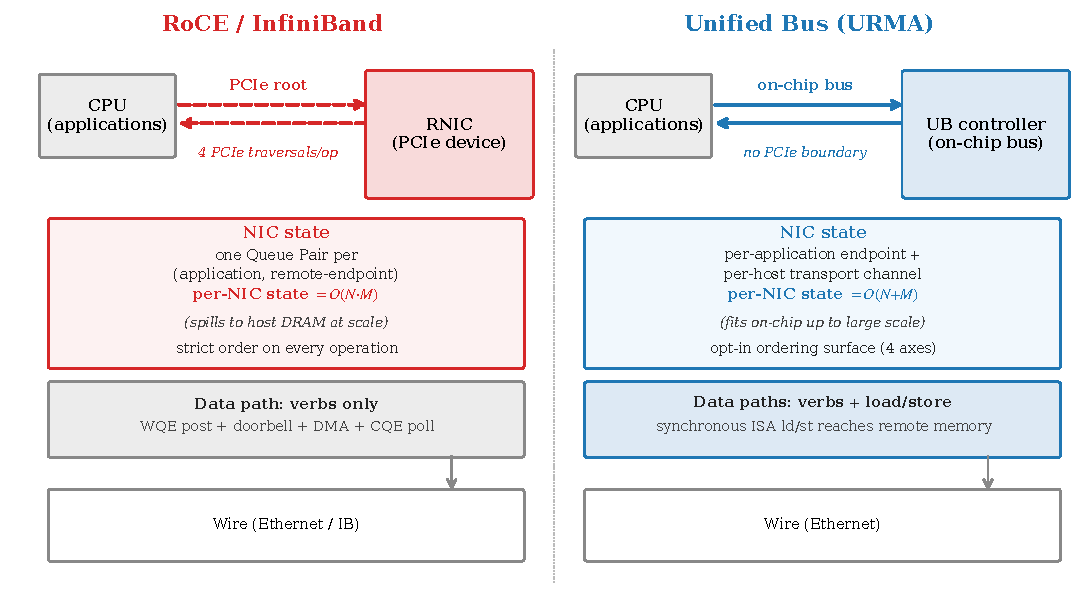
\includegraphics[width=0.95\textwidth]{figures/fig_arch_comparison.pdf}
  \caption{Architectural comparison. RoCE puts the NIC behind PCIe;
  it holds one Queue~Pair per (application, remote-endpoint) pair,
  enforces strict order on every operation, and admits only the
  verb-driven data path. Unified Bus puts the controller on the
  on-chip bus; it holds per-application endpoint state separately
  from per-remote-host transport state, exposes ordering as an
  opt-in surface, and admits CPU load/store as a synchronous data
  path alongside the verb path.}
  \label{fig:arch-comparison}
\end{figure*}

\paragraph{State: split transaction layer from transport layer.}
The architectural insight that drives everything else is that the
QP's fusion of transaction-layer and transport-layer responsibilities
was a textbook layering violation that paid off only while the
quadratic state cost stayed small. UB undoes the fusion explicitly:
the transaction layer's responsibilities --- application identity,
work queues, completion delivery, permissions --- live on a
per-application object called a \emph{Jetty}, while the transport
layer's responsibilities --- sequence numbers, retransmit window,
in-flight bitmap, RTO timer, congestion-control state --- live on a
per-remote-host object called a \emph{TP~Channel}
(Figure~\ref{fig:state-model}). A Jetty carries $\sim$80~B of state
that scales as $O(N)$ in the local application count; a TP~Channel
carries $\sim$30~B of state that scales as $O(M)$ in the
remote-host count. Any Jetty can address any remote endpoint
through the per-host TP~Channel pool, with the destination Jetty
carried in the packet header rather than baked into a per-pair
binding. Total state grows as $O(N{+}M)$ by construction: at
$(N,M){=}(1024,1024)$, roughly 110~KB instead of 537~MB. The
quadratic count never appears because the abstraction never
asks for it.

The trade-off the split pays is one extra layer of indirection in
the NIC pipeline (an outbound packet must look up which TP~Channel
to ride on by destination host) and a protocol surface that exposes
Jetty and TP~Channel as separate first-class objects with separate
lifecycles. The QP's simplicity --- one object per peer, one
lifecycle to manage --- is the cost of admission. The payoff is that
the connection working set fits on the on-chip bus's locality budget
at scales that force RoCE to spill to host DRAM, which in turn
unlocks the on-chip-bus controller of the data-path choice below.

\begin{figure*}[t]
  \centering
  \includegraphics[width=0.95\textwidth]{figures/fig_state_model.pdf}
  \caption{State models compared. RoCE binds one Queue~Pair to every
  (application, remote-host) pair, so per-NIC state grows as
  $O(N{\cdot}M)$. UB decouples per-application state (Jetty) from
  per-host transport state (TP~Channel); any Jetty addresses any
  remote endpoint through the shared TP~Channel pool, and per-NIC
  state grows as $O(N{+}M)$.}
  \label{fig:state-model}
\end{figure*}

\paragraph{Ordering: an opt-in surface.}
RoCE~RC enforces strict in-order delivery on every operation: the
NIC retires completions in issue order even when the application
asked for two writes that happen to be independent. UB exposes
ordering as four orthogonal axes that the application opts into
per-channel and per-operation:

\begin{itemize}\itemsep 1pt
\item \textbf{Service mode (per channel)} controls how aggressively
the NIC may reorder packets on the wire. The relaxed mode admits
multi-path spreading; the strict mode forces single-path,
sequence-number-preserving delivery; intermediate modes trade
relaxation for retransmit cost.
\item \textbf{Execution order (per operation)} controls whether the
issue stage may emit the next operation before the previous one
commits, or must wait. Independent operations are tagged for
parallel emission; dependent ones for serial emission.
\item \textbf{Fence} is an explicit application-level barrier
serialising subsequent operations against all prior in-flight ones.
\item \textbf{Completion order (per operation)} controls whether
the completion queue retires entries in arrival order or in issue
order.
\end{itemize}

A pure-fanout broadcast bypasses every gating stage. A
barrier-after-collective pays exactly the gating its workload
needs. The trade-off UB pays is that the NIC pipeline must hold
the gating machinery for all four axes even when only one is in
use; the trade-off it avoids is paying the strict-order tax on
every operation regardless of need.

There is a second, less obvious argument for opt-in ordering that
the failure model surfaces. Enforcing a single global order on every
operation is not only expensive on the fast path; it is also fragile
under failure. A NIC that has promised in-order delivery on every
in-flight operation cannot retire any completion if any earlier
operation has stalled, so a single slow path becomes a
head-of-line block for every application sharing the channel.
Modern AI-training workloads tolerate the relaxed contract by
construction (gradient updates are approximate; many independent
parameters can be exchanged in any order), and the workloads that
do need a barrier --- a fence after a collective, a strict-order
write after a flush --- can request exactly that one barrier without
imposing the cost on every other operation. The graded surface
reflects what the workloads actually need, not what the protocol
finds easiest to guarantee.

\paragraph{Data path: load/store on the on-chip bus.}
For small synchronous operations, UB defines an alternative data
path in which the CPU issues bare load and store instructions to
an address aperture owned by a controller on the on-chip bus
(Figure~\ref{fig:dataflow-comparison}). The controller translates
each instruction into a single-shot network transaction with no
work-queue entry, no doorbell, no DMA, and no separate completion
message: the load instruction blocks until the response data
returns. The four PCIe traversals of the work-queue-driven path
collapse into on-chip-bus crossings roughly an order of magnitude
smaller.

The trade-off this path pays is that the controller must sit on
the same on-chip-bus segment as the CPU it serves --- the operation
is synchronous, so it cannot ride over PCIe distance without losing
its latency advantage --- and that only a subset of the protocol
surface is admissible (small loads and stores, plus atomics on the
same path; bulk transfers and async operations stay on the
work-queue-driven path). The trade-off it avoids is the PCIe round
trip itself, on the operations where avoidance matters most: small
synchronous accesses to remote memory, which is exactly the shape
of a CPU-issued remote read.

The load/store path does not replace the work-queue-driven path; it
\emph{complements} it. Synchronous CPU-issued accesses to small
remote memory are well served by load/store because the CPU's
critical path is short and the data fits in a register. Large bulk
transfers are well served by the work-queue path because the
issue-side cost amortises across many bytes and the CPU does not
need to block. The protocol offers both because the two cover
disjoint operating points: load/store wins where the operation is
short and the latency budget is tight; the work-queue path wins
where the operation is long and the throughput budget dominates.
A NIC that supports only one is a NIC that asks the application to
push the wrong shape of operation through the wrong abstraction.

\begin{figure*}[t]
  \centering
  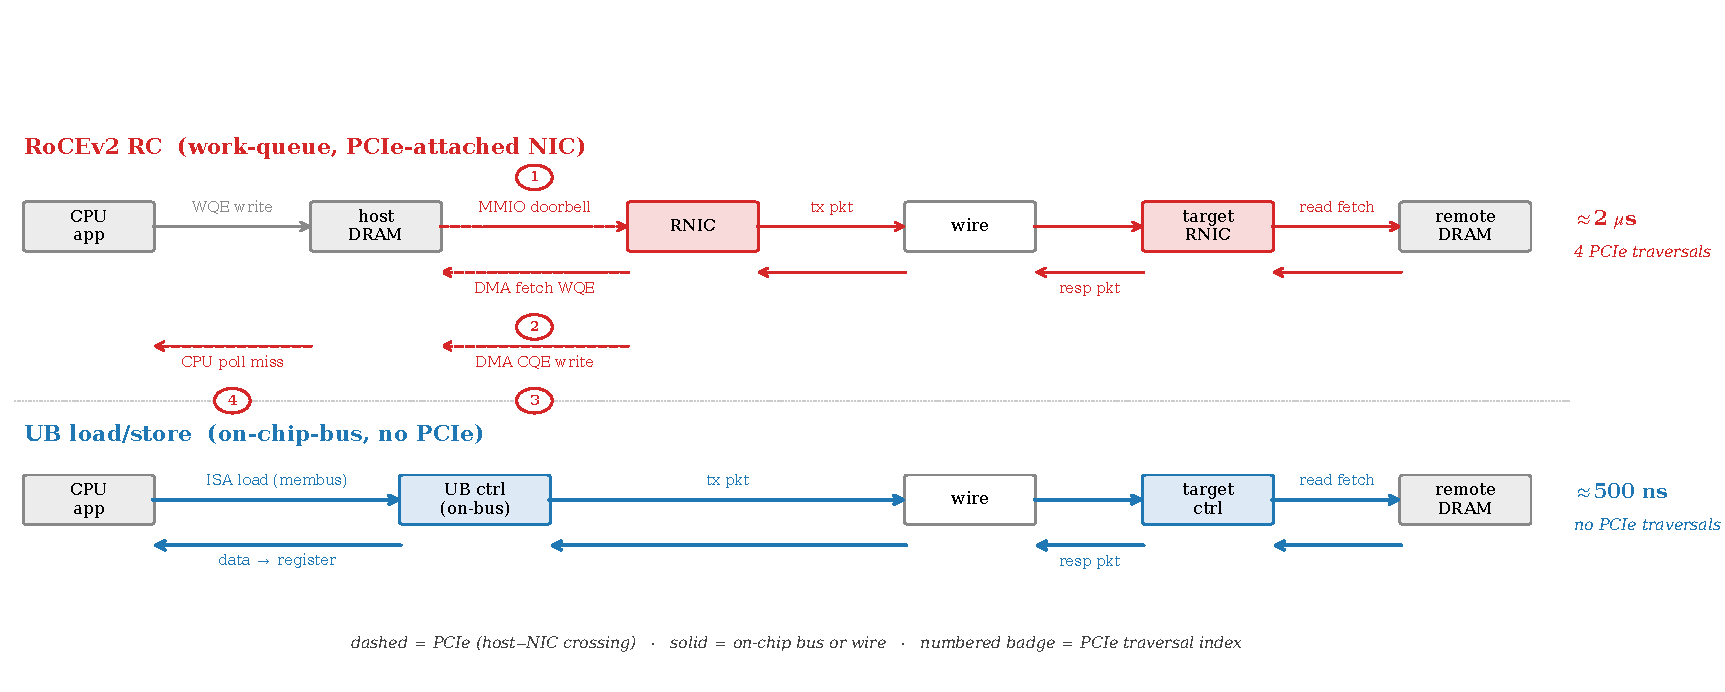
\includegraphics[width=0.95\textwidth]{figures/fig_dataflow_comparison.pdf}
  \caption{Per-operation data path for a small synchronous read.
  The traditional work-queue-driven path (top) traverses four PCIe
  crossings --- doorbell over MMIO, work-queue-entry DMA fetch,
  completion-entry DMA write, and a CPU poll-miss across PCIe
  coherence. The Unified Bus load/store path (bottom) replaces all
  four with on-chip-bus crossings: a CPU load instruction reaches
  the controller, the controller emits the wire packet, the
  response arrives, and the data lands directly in the CPU register
  that issued the load.}
  \label{fig:dataflow-comparison}
\end{figure*}

\subsection{The OpenClickNP toolchain}
\label{subsec:openclicknp}

OpenURMA is built on OpenClickNP~\cite{openclicknp}, a clean-room
re-implementation of the ClickNP element model~\cite{li2016:clicknp}.
The model is a familiar one: a NIC pipeline is a directed graph of
\emph{elements}, each with typed input and output ports, local
state, and a per-cycle handler. The toolchain lowers a single
source description through three back-ends: a software emulator
for unit testing, a cycle-accurate SystemC simulator for performance
measurement, and a Vitis~HLS back-end that emits synthesisable C++
for Vivado synthesis on the Alveo~U50. The same source produces all
three artifacts. The relevance to this paper is twofold: the model
makes element-level cost (LUTs, pipeline-II, BRAM) directly
measurable, and the three back-ends are how OpenURMA produces both
the RTL tier and the SystemC tier from one description.

\section{Design}
\label{sec:design}

This section describes how OpenURMA realises Unified Bus in RTL. We
organise the description around the three architectural commitments
introduced in \S\ref{subsec:ub-changes} --- bounded state, opt-in
ordering, and the load/store data path --- followed by the
composition that makes the three mutually load-bearing. The
element-by-element decomposition, port wirings, and HLS-pragma
specifics are deferred to \S\ref{sec:impl}; this section keeps the
discussion at the level of how the pipeline embodies each
architectural choice and what trade-offs that embodiment forces.

\begin{figure*}[t]
  \centering
  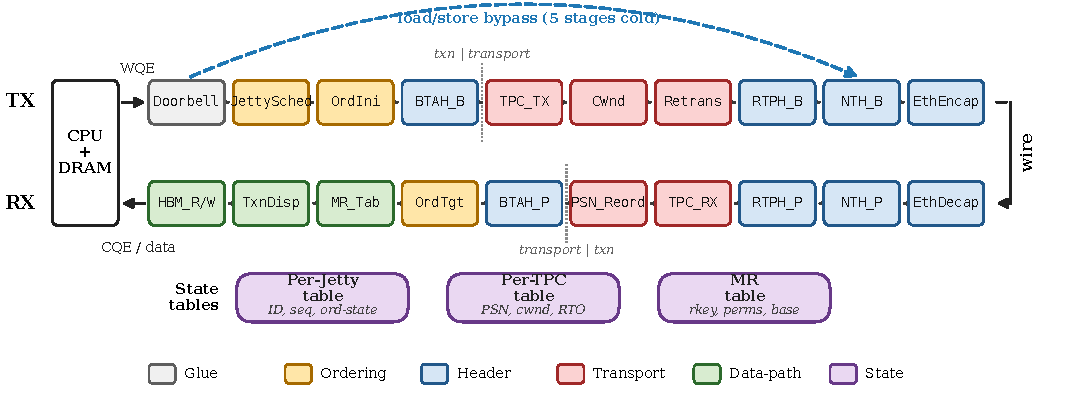
\includegraphics[width=0.95\textwidth]{figures/fig_pipeline_topology.pdf}
  \caption{OpenURMA's NIC pipeline, organised by protocol layer. The
  transaction layer (top half) handles application-level concerns ---
  Jetty scheduling, ordering, memory-region checks, atomic operations,
  completion generation. The transport layer (bottom half) handles
  per-host concerns --- packet sequence numbers, retransmission,
  congestion control, multi-path. The two layers communicate through
  flit-typed boundaries; the load/store data path
  (\S\ref{subsec:design-loadstore}) bypasses the transport layer
  entirely.}
  \label{fig:topology}
\end{figure*}

\subsection{Realising bounded state}
\label{subsec:design-state}

The state model from \S\ref{subsec:ub-changes} --- per-application
Jetty objects plus per-host TP~Channel objects, with any-to-any
addressing through the shared TP~Channel pool --- maps onto two
pipeline regions. The transmit path consults a per-Jetty state table
to admit and gate work-queue entries from the local application,
then hands each request to a per-host TP~Channel scheduler that
attaches the right sequence number, picks the multi-path lane, and
queues the packet for transmission. The receive path inverts the
flow: the per-TP-Channel logic validates and reorders packets by
sequence number, then a per-Jetty table maps the destination header
to the right local application's receive queue. Two tables, two
indices, two scaling regimes.

The implementation cost of the split is one extra header field in
every transmitted packet to carry the destination application's
identifier, and one extra table lookup on each side of the wire to
turn that identifier into a Jetty pointer. The implementation
saving --- and the architectural payoff --- is that nothing in the
pipeline binds a transmit context to a receive context. A Jetty
can address every remote endpoint it has permission for through the
same per-host TP~Channel, with no per-pair state created and no
per-pair lifecycle to manage. The protocol's $O(N{+}M)$ scaling is
the pipeline's; the table sizes follow.

A consequence of bounded state is that the entire connection
working set --- per-Jetty state plus per-host TP-Channel state ---
fits in on-chip BRAM at scales that would force RoCE to host DRAM.
At $(N,M){=}(1024,1024)$, OpenURMA's two-table working set is
$\sim$110~KB; the same workload's RoCE QP table is $\sim$537~MB.
We return to this measurement in \S\ref{subsec:state-decomp}.

\subsection{Realising opt-in ordering}
\label{subsec:design-ordering}

The four-axis ordering surface from \S\ref{subsec:ub-changes}
becomes four pipeline structures. Each axis decides at one
well-defined stage whether the operation in flight may proceed
or must wait; together they form a gating mesh that any operation
traverses, but the mesh adds zero pipeline cycles to operations
whose mode bypasses all four. The trick is what the gating logic
indexes against.

\paragraph{The reused-counter argument.}
Each gating decision in the ordering surface requires the same
inputs: a per-application sequence-number counter (for the
``do prior operations from this application still need to
complete?'' check), a per-channel outstanding-window counter
(for the ``can the wire absorb another operation?'' check), and
a per-application fence latch. These three counters are already
required by the state model in
\S\ref{subsec:design-state} --- the per-Jetty table holds them
either way, because the spec defines the relevant sequence numbers
as per-Jetty objects. The ordering surface reads from the same
counters the state model writes to; it does not add a parallel
bookkeeping structure. This is what makes opt-in ordering cheap:
the per-Initiator machinery the four modes select among is
provisioned by the layer split, not added on top of it.

\paragraph{Two reorder buffers, not one.}
A subtler choice is that the pipeline carries \emph{two} reorder
buffers serving disjoint correctness contracts
(Figure~\ref{fig:two-reorder}). One acts at the transport layer
on packet sequence numbers and delivers byte-correct flits to the
upper layer regardless of any application's ordering choice; this
is what lets a single TP~Channel multiplex traffic from multiple
applications without one application's wire-byte gaps stalling
another's. The other acts at the transaction layer on per-application
sequence numbers and delivers in-application-order completions
regardless of wire-byte order; this is what lets the transmit path
spread an application's packets across multiple network paths
without breaking the application's view that completions arrive
in issue order.

Collapsing the two into one couples the contracts: every
multi-path-induced packet gap would block the completion stream;
every per-application dependency stall would back-pressure the
wire. The separation is what makes the unordered service mode
correctness-safe at the same time as the strict mode, and it is
what makes multi-path spreading a first-class feature rather than
a correctness hazard. We return to this design choice in
\S\ref{sec:related} where we contrast it with the per-transaction
bitmap-tracked alternatives that UEC~\cite{uec2025:spec} and
MP-RDMA~\cite{lu2018:mprdma} take.

\begin{figure*}[t]
  \centering
  \includegraphics[width=0.95\textwidth]{figures/fig_two_reorder_buffers.pdf}
  \caption{The pipeline carries two reorder buffers serving disjoint
  correctness contracts. Packet-sequence reordering at the transport
  layer delivers byte-correct flits regardless of application
  ordering; transaction-sequence reordering at the transaction layer
  delivers in-issue-order completions regardless of wire-byte order.
  The separation is what makes multi-path spreading and opt-in
  ordering composable.}
  \label{fig:two-reorder}
\end{figure*}

\subsection{Realising the load/store path}
\label{subsec:design-loadstore}

The load/store data path is the most architecturally distinctive
part of OpenURMA, because it is the first part where ``put the NIC
on the on-chip bus'' becomes ``what does the NIC pipeline actually
look like.'' The work-queue-driven path described above carries
ten pipeline stages cold (work-queue scheduling, ordering, header
build, transport accounting, congestion check, multi-path lane
selection, retransmit-buffer write, framing, transmit). For a small
synchronous operation, every one of those stages is overhead the
abstraction does not need.

The load/store path drops them. A CPU \texttt{ld} or \texttt{st}
instruction to the address aperture owned by the controller emerges
at a single stage that builds the transaction header, attaches a
flag declaring transport-layer bypass, builds the network header,
and frames the packet for the wire --- five stages cold total. No
work-queue entry is written, no completion entry is written, no
sequence number is allocated (the bypass flag tells the receiving
NIC to skip its transport-layer state machine), no retransmit
buffer slot is held (the protocol falls back to the CPU's load
re-issue on timeout, which is cheaper than maintaining
transport-layer reliability for an operation that takes the
synchronous path anyway). The trade-off is the one stated in
\S\ref{subsec:ub-changes}: the path admits only operations whose
semantics survive transport bypass --- small loads, stores, and
atomics on the same memory --- and the controller must be on the
same on-chip-bus segment as the CPU. Bulk transfers and async
operations stay on the work-queue-driven path because their
latency budget tolerates the ten stages.

\subsection{Hardware fanout: target-side dispatch}
\label{subsec:design-fanout}

A second consequence of bounded state is that the target-side
demultiplexing logic --- the step that decides which local
application receives an incoming SEND --- can live in
hardware rather than in a CPU event loop. RoCE handles this in
software: the target NIC writes a completion to a shared queue,
the application event loop polls, and the dispatch happens at
CPU speed. UB defines a \emph{Jetty Group} construct in which a
single externally visible identifier represents a set of member
Jetties, and the receiving NIC dispatches incoming SEND
operations to one of the members in hardware under one of three
policies (hashing on an Initiator-supplied key, round-robin, or
load-balancing by receive-queue depth)
(Figure~\ref{fig:jetty-group-arch}).

The architectural payoff is that the target CPU is not on the
SEND fast path. The trade-off is one extra pipeline
element on the RX path between transaction dispatch and the
per-Jetty receive logic, with per-group state on the order of
$\sim$80~B for a 8-member group. We measure the end-to-end
saving in \S\ref{subsec:m2n}: ${\sim}200$~ns per SEND
when the fanout is small, growing to ${\sim}1200$~ns once the
RoCE side begins paying for QP-state spill on top of the CPU
dispatch.

\begin{figure*}[t]
  \centering
  \includegraphics[width=0.95\textwidth]{figures/fig_jetty_group_arch.pdf}
  \caption{Target-side SEND dispatch. RoCE demultiplexes
  through a shared completion queue plus an application event loop;
  UB's Jetty~Group performs the dispatch in hardware on the
  membus crossing already paid for by NIC RX.}
  \label{fig:jetty-group-arch}
\end{figure*}

\subsection{How the three commitments compose}
\label{subsec:design-composition}

The implementation makes visible a coupling the introduction
asserted but could not justify in detail there: each of UB's three
architectural commitments depends on the others being present.

\paragraph{The on-chip controller depends on bounded state.}
The load/store path of \S\ref{subsec:design-loadstore} lives on
the on-chip bus because it does not need DRAM access to look up
the per-application state required to authorise the operation;
the bounded state of \S\ref{subsec:design-state} keeps that state
in on-chip BRAM. If state spilled to host DRAM, the controller
would have to issue an external memory access on every load/store,
which would put it back in PCIe-latency territory and defeat the
point of the on-bus placement.

\paragraph{Opt-in ordering depends on the layer split.}
The gating logic of \S\ref{subsec:design-ordering} reads counters
the per-Jetty table already provides; the gating logic costs
roughly 13~KLUT (10.6\% of the design's LUT budget) and
\emph{zero} added pipeline cycles on operations whose mode
bypasses gating. If the state model had not split per-application
from per-host state --- if the design had remained QP-centric ---
the ordering surface would have to add the per-application
counters from scratch, and the cost would compound on every
operation regardless of need.

\paragraph{Multi-path spreading depends on the two-reorder split.}
The unordered service mode authorises a transmit path to spray
packets across multiple wire paths for bandwidth and resilience.
The split between transport-layer and transaction-layer reordering
(\S\ref{subsec:design-ordering}) is what makes that spreading
correctness-safe without per-transaction SACK metadata: an
unordered application receives unordered completions; an ordered
application sharing the same wire receives ordered completions;
neither stalls the other. Collapsing the buffers would force one
contract onto both.

These dependencies are why we say the three commitments are three
faces of one architectural commitment. The next two sections show
what that commitment costs (\S\ref{sec:impl}) and what it saves
(\S\ref{sec:correctness} onwards).

\section{Implementation}
\label{sec:impl}

This section opens the implementation up to the level of detail the
design discussion deliberately deferred. We describe the pipeline
decomposition, the two new pipeline elements introduced for the
load/store path and target-side fanout, the toolchain extensions,
the multi-tier simulation infrastructure (SystemC and gem5), and
the timing-closure sweep that produced the 322~MHz post-route
result. Throughout, we describe what each piece \emph{does} rather
than what its source file is named; the implementation is open and
source-level identifiers are what they are at the time of writing,
but the protocol responsibilities the implementation maps onto are
stable.

OpenURMA is roughly 3.5~KLOC of element-level source spread across
39 pipeline elements implementing the transport and transaction
layers. The parallel OpenRoCE baseline (RoCEv2~RC) is roughly
1.3~KLOC across 21 elements. Both stacks sit on the same
OpenClickNP toolchain~\cite{openclicknp}, so all measurements
compare implementations produced by an identical lowering pipeline.

\subsection{Pipeline decomposition}
\label{subsec:impl-elements}

The 39 OpenURMA pipeline elements break into six functional
categories. The counts and responsibilities are what the protocol
requires.

\begin{itemize}\itemsep 1pt
\item \textbf{10 header parsers and builders} handle the four
  layered headers the spec defines --- Ethernet framing, a
  network-transport header, a reliable-transport header, an
  unreliable-transport variant, and a base-transaction header ---
  as matched parser/builder pairs.

\item \textbf{9 transport-layer elements} implement the per-host
  TP~Channel pipelines on both ends, the retransmission buffer,
  the packet-sequence reorder buffer, the two
  acknowledgement-generation elements (one for the lower layer's
  per-packet acks, one for the upper layer's transaction-level
  acks), the congestion-control window, the congestion-echo
  feedback element, and the multi-path transport-protocol-group
  dispatcher.

\item \textbf{4 ordering elements} implement the gating surface
  introduced in \S\ref{subsec:design-ordering}: the Jetty
  scheduler at admission, two order trackers (one each at the
  initiator and the target, because the gating responsibility
  shifts between endpoints depending on the service mode), and a
  transaction-layer completion reorder buffer.

\item \textbf{7 data-path elements} handle on-NIC memory reads and
  writes, atomic operations, per-Jetty receive logic, the new
  target-side dispatcher (\S\ref{subsec:impl-newelements}), the
  transaction dispatch-by-opcode router, and the completion
  generator.

\item \textbf{3 state tables} hold the memory-region permissions,
  the per-Jetty state, and the per-TP-Channel state.

\item \textbf{6 glue elements} provide the doorbell, dispatch
  multiplexers, completion notification tees, completion-queue
  streamers, and the retransmission RTO timer.
\end{itemize}

Three pipeline-decomposition choices deserve note. The
initiator-side and target-side order trackers are distinct elements
because the gating responsibility moves between endpoints depending
on the service mode (the relaxed mode places it at the target; the
strict mode places it at the initiator). The transaction-layer
completion reorder buffer is a distinct element rather than a flag
on the per-Jetty receive logic because the
in-order-versus-arrival-order choice is per-operation and requires
a per-application sliding window, not a per-Jetty mode bit. The
packet-sequence reorder buffer is distinct from the
transaction-layer completion reorder buffer for the two-buffer
reason discussed in \S\ref{subsec:design-ordering}: the two serve
disjoint correctness contracts on disjoint sequence-number spaces.

The transmit path threads through ten pipeline stages cold for the
work-queue-driven path: doorbell admission, Jetty scheduling,
initiator-side ordering check, base-transaction-header build,
TP-Channel transmit logic, congestion-window check, retransmission
buffer write, reliable-transport-header build,
network-transport-header build, and Ethernet encapsulation. The
receive path inverts the sequence. The full topology is in
Figure~\ref{fig:topology}.

\subsection{Two new pipeline elements}
\label{subsec:impl-newelements}

Two pipeline elements are not derivable from existing OpenClickNP
templates and required new design.

\paragraph{The load/store transport-bypass engine.}
The five-stage transport-bypass pipeline introduced in
\S\ref{subsec:design-loadstore} is implemented as a single new
element threaded into a separate topology variant alongside the
default work-queue-driven topology. The transmit handler accepts a
load or store doorbell request from the on-chip-bus side, allocates
a one-shot transaction context (no per-channel sequence-number
allocation, no retransmission-buffer slot), stamps a
transport-bypass flag in the next-layer-protocol field so the
receiving NIC skips its transport state machine, and frames the
packet. Posting a single load request, the first wire flit emerges
at \textbf{8 cycles ${\approx}25$~ns at 322~MHz} --- 17 cycles
($\approx$53~ns) below the work-queue-driven path on identical
infrastructure. The saving is the protocol-layer instantiation of
spec-mandated transport bypass; it is not microarchitectural.

\paragraph{The target-side hardware dispatcher.}
The target-side hardware dispatcher introduced in
\S\ref{subsec:design-fanout} sits between transaction dispatch and
the per-Jetty receive logic on the RX path. When an incoming
SEND addresses a registered Jetty-Group identifier, the
element rewrites the extension flit's destination field to point at
one of up to eight member Jetties according to a per-group policy:
\emph{hint-hash} (the member index is the application-supplied hint
modulo the member count, which lets the initiator steer requests
by an opaque key as long as the application chooses the key
consistently), \emph{round-robin} (a cursor advances per
SEND), or \emph{receive-queue-depth load balancing} (the
member with the shallowest pending receive-queue depth wins).
SENDs to unregistered identifiers pass through unchanged,
so the element is opt-in per group. Per-group state is on the
order of $\sim$80~B for a maximum-membership (8-member) group: one
identifier and two counters per member, plus a small header.

\subsection{Retransmission and congestion control}
\label{subsec:impl-retrans}

The retransmission buffer is a 64-slot in-flight ring per
TP-Channel with both Go-Back-N and selective-retransmit modes.
The selective-retransmit path uses the spec-defined selective-ack
response opcode plus a per-PSN bitmap in the acknowledgement
header. The retransmit decision is driven either by a
transaction-layer acknowledgement that explicitly NAKs PSNs
(selective) or by the RTO timer firing (Go-Back-N). Each slot
captures one metadata-and-extension flit pair, which is sufficient
for control-plane work requests and for $\le$8-byte Writes. \emph{Multi-flit retransmission} --- extending the slot to a
payload-flit list so a dropped multi-flit Write can be replayed in
full --- is implemented in the loss-free Write data path
(\S\ref{sec:correctness}) but not yet in the retransmit buffer; we
flag this in \S\ref{sec:discussion}.

The congestion-control loop combines a host-side switch model with a
per-channel additive-increase / multiplicative-decrease window. The
switch is a SystemC and software-emulator element
that maintains a queue with low/high watermarks and stamps the
forward explicit congestion-notification bit on packets when
occupancy crosses the high watermark. The Initiator-side
the congestion-window element listens for marked acknowledgements and
applies a multiplicative decrease; absent marks, it additively
increases per RTT. The closed loop is verified in
the closed-loop test: 200 work requests
posted, 9 of the 25 packets that traverse the switch are marked,
and the sender's window drops from 65{,}536~B to 4{,}096~B in
response.

\subsection{Toolchain extensions}
\label{subsec:impl-dsl}

Six pipeline elements needed pipeline-initiation-interval guidance
to close 322~MHz; the back-end previously hard-coded $II{=}1$,
which over-pipelines elements whose data dependencies cannot be
unrolled aggressively. We added two pragma blocks to the
element-source grammar: one that lets an element declare its
initiation interval ($II$) explicitly, and one that lets an element
forward arbitrary HLS pragmas verbatim. Both extensions are
upstream in OpenClickNP and reused unchanged by both stacks. They
are the only modifications we made to the framework.

\subsection{Three back-ends from one source}
\label{subsec:impl-backends}

OpenClickNP lowers each \texttt{.clnp} element through three
back-ends. The first is a software emulator that wraps each
element's per-cycle handler in a a thread connected to
bounded SPSC FIFOs; this is the back-end the correctness tests of
\S\ref{sec:correctness} run against. The second is a cycle-accurate
SystemC simulator with a 1~ns clock period matching the 322~MHz
synthesis target, so a SystemC cycle count is directly comparable to
post-route Vivado timing; this is the back-end the microbenchmarks
of \S\ref{sec:sc} use. The third is a Vitis HLS back-end
that emits synthesisable C++, which Vivado then synthesises and
places-and-routes to a chosen Xilinx part; this is what produces the
LUT, BRAM, and timing numbers of \S\ref{sec:vivado}. All three
back-ends consume the same \texttt{.clnp} source, so an element
that closes timing in HLS corresponds exactly to the element the
SW emulator tested and the SystemC simulator benchmarked.

\subsection{Two-node SystemC simulator}
\label{subsec:impl-twonode}

The two-node simulator links each NIC stack as a static SystemC
library and wires two instances of each side through a SystemC
EtherLink module with configurable bandwidth and propagation delay.
Each endpoint is a full system: a CPU host model that constructs
work-queue entries and posts doorbells, the NIC's transmit and
receive pipelines, a DDR4 DRAM model for both work-queue-side and
data-side accesses, a two-level write-back / write-through /
uncached cache hierarchy for the host CPU, and a completion-queue
write-back path. The harness produces a 388-configuration sweep
covering all six verb categories, four cache policies, payload
sizes from 8~B to 4~KB, and link delays from 100~ns to 10~$\mu$s.

\subsection{gem5 full-system scaffold}
\label{subsec:impl-gem5}

For the CPU-to-remote-DRAM end-to-end claim, we integrate the
SystemC NIC into gem5 as a memory-mapped device. The integration
required three load-bearing changes against the current gem5
release.

\paragraph{SystemC ABI rebuild.}
Gem5 ships its own embedded SystemC headers; the upstream Accellera
SystemC build the OpenClickNP cycle-accurate back-end uses is
ABI-incompatible with them. We rebuild the NIC SystemC libraries
against gem5's headers, with a separate output target, and point
the gem5 build script there.

\paragraph{Port wiring and address-range partition.}
Gem5's memory-bus crossbar cannot route overlapping address ranges,
so the NIC's address aperture must be carved out of the system
memory range that the standard configurations use by default. The
controller's initialisation entry point must also explicitly call
the crossbar's range-change hook so the bus's address-range latch
settles before gem5's binary loader issues its first write through
the port proxy.

\paragraph{Dual-node configuration.}
A dual-node configuration brings up two ARM CPU instances with the
SystemC EtherLink between their controllers, runs a small set of
SE-mode binaries on each that exercise the NIC's address aperture
through ordinary load and store instructions, and pre-maps the NIC
aperture into each process's page table after binary load so the
CPU's loads and stores reach the controller without going through
gem5's full virtual-memory subsystem. The current scaffold validates
the end-to-end CPU-to-remote-controller path with SE-mode workloads;
full-system Linux integration is follow-on work.

\subsection{Timing-closure sweep}
\label{subsec:impl-closure}

The initial Vitis-HLS pass on the 38 work-queue-driven elements
left 8 elements needing remediation: 5 missed 322~MHz in Vivado
P\&R and 3 failed at HLS itself before reaching P\&R. The
mechanical resolution combined the new $II$ and HLS-pragma
extensions described above with a few targeted algorithmic
redesigns, summarised by element function in
Table~\ref{tab:timing-closure}.

\begin{table}[h]
  \centering
  \scriptsize
  \begin{tabular}{lll}
  \toprule
  Element function & Before $\to$ After (ns WNS) & Action \\
  \midrule
  Atomic operations           & $-1.871 \to +0.298$ & $II{=}4$ + memory partition \\
  Completion reorder          & HLS-stuck $\to +0.672$ & head-pointer ring + $II{=}2$ \\
  Initiator order tracker     & $-5.382 \to +0.318$ & $II{=}2$ \\
  Jetty scheduler             & HLS-aborted $\to +0.546$ & $II{=}2$ \\
  Target order tracker        & $-2.25 \to +0.101$ & $II{=}2$ + drain re-order \\
  On-NIC memory write         & $-0.628 \to +0.628$ & memory partition \\
  Memory-region table         & failing $\to +0.729$ & shrink table to 64 entries \\
  On-NIC memory read          & $-0.449 \to +0.282$ & word-sized array \\
  \bottomrule
  \end{tabular}
  \caption{Timing-closure remediation, by element function.}
  \label{tab:timing-closure}
\end{table}

\paragraph{One instructive failure.}
The most instructive case is the on-NIC memory-read element, which
originally backed its 64~KB read path with a byte-sized array plus
cyclic memory partition for parallel byte-bank access. HLS
estimated 490~MHz F${}_{\max}$; Vivado P\&R reported $-0.449$~ns
WNS. The worst path ran from a register inside the per-bank index
computation into the BRAM address port of the partitioned array:
8 LUT levels of barrel-shift mux to compute the per-bank index,
plus 2.7~ns of routing delay (76\% of the period). No combination
of $II$ or partition factor moved the slack; the wide muxing for
the 8 banks bloated routing without unblocking timing. The fix was
algorithmic: replace the byte-sized array with an 8-byte-word-sized
array indexed by a shifted offset. Each 8-byte-aligned read becomes
a single BRAM word access; the byte-bank mux is gone; the memory
partition pragma is no longer needed. WNS closes at $+0.282$~ns.
The same pattern was applied to the OpenRoCE on-NIC memory-read
element. The lesson is that HLS's per-element timing estimate is a
useful but optimistic predictor; routing-bound paths only show in
Vivado P\&R, and the right resolution may be at the data-layout
level rather than the pragma level.

\subsection{Test coverage}
\label{subsec:impl-tests}

The 16 SW-emu integration tests (enumerated in
\S\ref{sec:correctness}) cover correctness across the spec surface,
the wire format, the closed congestion-control loop, the multi-flit
Write payload path, the fused-acknowledgement fusion, and the full
atomic opcode set. A sustained-throughput sanity check posts
50{,}000 work requests through the same harness. The SystemC
back-end runs a cycle-accurate latency benchmark that drives
requests through the entire transmit-to-wire-to-receive path and
reports first-flit latency, round-trip latency, and sustained
throughput. The HLS synthesis sweep and Vivado P\&R sweep are
scripted for one-button reproducibility.

\section{Evaluation Methodology}
\label{sec:methodology}

Because no FPGA is available for in-silicon experiments, we evaluate
the design through three independent paths, each answering a
different class of question:

\begin{itemize}
\item \textbf{SW-emulator (functional correctness).} Each
  \texttt{.clnp} element compiles to a C++ kernel that runs in a
  a thread with bounded SPSC FIFOs between elements.
  Tests post WRs into the pipeline's input stream, drain
  responses, and assert spec-defined behaviour.
\item \textbf{SystemC (cycle-accurate).} The same elements compile
  to per-element SystemC modules, one a 1-ns wait
  per loop iteration so that 1~ns of simulation time corresponds
  to one cycle at the 322~MHz target. We measure cycle counts directly
  and convert to wall-clock by multiplying by the post-route clock
  period (3.106~ns).
\item \textbf{Vivado synth$+$place$+$route (real RTL).} Each element's
  HLS-synthesised Verilog goes through a full Vivado out-of-context
  flow targeting the Alveo U50 (the Alveo U50 part). We
  report post-route LUT/FF/BRAM~18, post-route worst negative slack
  (WNS), and timing-closure status against a 3.106~ns clock period.
\end{itemize}

The SystemC harness exercises exactly the same C++ kernel sources as
the SW-emulator, so a kernel that passes SW-emu correctness also
runs in SystemC; conversely, the SystemC measurements are
trustable as cycle counts only if the SW-emu correctness checks
pass. Vivado synth runs on the HLS-emitted Verilog from the same
\texttt{.clnp} sources.

Every number in the rest of the paper is reproducible from the
released evaluation harness, which drives correctness, Vivado P\&R,
and the SystemC microbenchmark sweep end to end and writes all
results out as CSV.

\section{Functional correctness}
\label{sec:correctness}

Seventeen SW-emu tests cover the spec surface and the framework
internals; all pass on the current source tree.

\begin{itemize}
\item \textbf{Initiator-side ordering} --- a strict-order
  operation is gated behind a relaxed-order operation; the
  pipeline holds the strict op at the initiator until the
  relaxed one commits.
\item \textbf{Target-side ordering} --- the target serialises
  strict-order operations at execution time, deferring them
  behind missing prior operations.
\item \textbf{Fused acknowledgement} --- the lower-layer ack
  carries the upper-layer ack on the same flit, saving one wire
  packet per response under the fused-ack service mode.
\item \textbf{Fence} --- a fenced operation waits until all prior
  reads and atomics have responded before its own emission.
\item \textbf{Completion ordering} --- with the in-issue-order bit
  set, completions are retired in original-issue order; with it
  clear, they are retired in arrival order.
\item \textbf{Unordered Send wire path}.
\item \textbf{Mixed-mode operations} in the same send queue.
\item \textbf{Multi-initiator parallelism} --- per-initiator
  gating: a strict-order operation on one initiator emerges
  immediately while a strict-order operation on a different
  initiator is gated behind its own dependency.
\item \textbf{Head-of-line-blocking isolation} --- 8 unordered
  operations from 4 initiators all emerge despite a stalled
  strict-order operation on a separate initiator.
\item \textbf{On-NIC memory read/write data integrity}.
\item \textbf{Full atomic opcode set} ---
  swap, store, load, fetch-and-add, fetch-and-subtract,
  fetch-and-and, fetch-and-or, fetch-and-xor; each verified to
  return the pre-modification value in the response and to leave
  the on-NIC memory word in the algebraically correct
  post-state. Compare-and-swap is covered by the mixed-mode test.
\item \textbf{Transmit-to-wire round trip} with all UB header
  fields preserved.
\item \textbf{Sustained-throughput sanity} (50{,}000 work requests).
\item \textbf{Wire-format encoder} against the spec bit layout.
\item \textbf{End-to-end congestion-control loop} --- 200 work
  requests posted; 9 of the 25 packets that traverse the
  modeled switch are congestion-marked; the sender's congestion
  window backs off from 65{,}536~B to 4{,}096~B.
\item \textbf{Target-side hardware dispatch} --- the dispatcher
  routes incoming SENDs to one of $N$ member Jetties under three
  policies (hash on an application-supplied hint, round-robin,
  receive-queue-depth load balancing). The test exercises all
  three on a 4-member group plus the unregistered-identifier
  bypass; the end-to-end consequence is quantified in
  \S\ref{subsec:m2n}.
\item \textbf{Multi-flit Write payload path} --- 8/32/64/128/256-byte
  writes through Ethernet-encapsulation streaming, decapsulation
  reassembly, and the on-NIC memory-write payload byte stream.
\end{itemize}

\paragraph{What the SW-emu suite does \emph{not} cover.}
The eval as it stands exercises every implemented mode and opcode
on the loss-free path. It does \emph{not} cover the loss path for
multi-flit Writes: the retransmit buffer slot stores one (meta, ext)
pair, so Go-Back-N or SACK replay of a dropped multi-flit Write
would not currently re-issue the payload bytes. Enabling that
requires extending the retrans slot to a payload-flit list (a
follow-on work item, \S\ref{sec:discussion}). All single-flit retransmit
paths (control-plane WRs, $\le 8$~B Writes, Reads, Atomics) are
exercised by the C-AQM closed-loop test through Cong\_Echo, but
explicit drop-injection tests remain follow-on work.

\section{Cycle-accurate microbenchmarks}
\label{sec:sc}

We instrument the TX pipeline (the harder of the two paths to reason
about, since it is where the ordering surface sits) under several
SystemC scenarios. Each scenario runs as one
SystemC microbenchmark invocation and writes one CSV row per
parameter point.

\subsection{Per-stage latency breakdown}
A single Write WR (ROL+NO) drives the pipeline cold. Tap monitors
inserted between every adjacent stage record the first-flit arrival
time. Figure~\ref{fig:per_element_latency_a} shows the per-stage
contribution.

The slowest stages are the Jetty scheduler (5 cycles --- $II{=}2$
plus the per-Initiator round-robin scan) and Ethernet encapsulation
(11 cycles --- byte-stream-rate, not flit-rate). The
initiator-side order tracker costs 1 cycle on the unblocked path:
the gating logic adds combinational depth (covered in
\S\ref{sec:vivado}) but no extra pipeline cycles when no prior
dependencies are outstanding. Total cold-path TX latency: 24
cycles $\approx$ 75~ns at 322~MHz.

\subsection{Per-mode TX latency}
We sweep all 4 service modes $\times$ 3 execution tags = 12 combinations
on the same single-WR cold path. \emph{Result: every combination
emits the first wire flit at exactly 24 cycles.} The per-mode
penalty is therefore not in pipeline-stage count but in the
combinational logic depth of each kernel — and that is what shows
up in the Vivado area report (\S\ref{sec:vivado}), not in the SystemC cycle count.
This is the design's intended behaviour: opt-in ordering does not
add pipeline cycles when not used.

\subsection{Sustained throughput per service mode}
A burst of 256 WRs (NO tag, varying service modes) is posted into
the doorbell input. Steady-state throughput is calculated as
$(N{-}1)/(\Delta t)$.

\begin{table}[h]
  \centering
  \footnotesize
  \begin{tabular}{lr}
  \toprule
  Service mode & Steady WR/$\mu$s \\
  \midrule
  OpenURMA: ROI / ROT / ROL / UNO & \textbf{150.36} \\
  OpenRoCE RC (matched microbench) & 53.62 \\
  \bottomrule
  \end{tabular}
\end{table}

All four OpenURMA service modes share a single transmit pipeline
(the unordered mode bypasses sequence-number allocation within the
TP-Channel transmit element but still traverses the same kernel
chain), and the throughput floor is set by the slowest pipeline
initiation interval in the chain ($II{=}2$ in the Jetty scheduler,
the initiator-side order tracker, the completion reorder buffer,
and the target-side order tracker; $II{=}4$ in the atomic-operation
element). Hence the per-mode rate is identical at 150.36~WR/$\mu$s.
The OpenRoCE baseline runs the matched-shape microbenchmark on
identical infrastructure and measures 53.62~WR/$\mu$s ---
\textbf{2.80$\times$ slower} --- because RC's per-QP sequence-number
allocation introduces stricter inter-operation dependencies in the
QP transmit kernel. The 1000-WR burst-saturation regime reaches
159.46~WR/$\mu$s on OpenURMA and 53.65~WR/$\mu$s on OpenRoCE; the
burst number trades extra cold-path cycles for higher steady-state
when the pipeline runs maximally saturated.

\subsection{Ordering surface: Fence and serialised-order gating cost}
We isolate the \emph{cost of gating itself} (independent of network
RTT) by injecting completion notifications synchronously and
measuring the cycles between completion and the gated WR's emission.
Figure~\ref{fig:gating_a} plots both costs.

\begin{itemize}
\item \textbf{Fence (Jetty\_Sched, \S7.3.2.2 note).} Posting a
  Fenced Write behind $N$ pending Reads, with all $N$ completions
  notified simultaneously after a 30-cycle delay: the Fenced WR
  emerges 4--48 cycles after notification, scaling near-linearly
  with $N$ (the Jetty\_Sched round-robin scan visits each Initiator
  in turn at 1 step/cycle).
\item \textbf{SO (OrderTracker\_Initiator, \S7.3.3.2).} Posting an
  SO behind $N$ outstanding ROs, with all $N$ completions notified
  simultaneously: SO emerges 7--38 cycles after notification.
  The cost is bounded by ord\_ini's 16-position round-robin cursor.
\end{itemize}

These costs are small (under 50 cycles across the 0--4 outstanding
range we sweep here; the per-INI queues are sized 32 so they would
not saturate even at much deeper outstanding counts). Crucially,
they are paid only when gating is requested; an application that
uses NO+UNO sees neither.

\subsection{Cross-INI head-of-line isolation}
We force one Initiator (rc\_id 0xA) into a permanent ROI+SO stall
by emitting an RO and then a gated SO whose RO completion is never
notified. We then post 8 UNO+NO WRs from four different Initiators
(0xB0..0xB3). Figure~\ref{fig:hol} shows that all 8 stream-B WRs
emerge at the wire within 78 cycles of post — they bypass the
gating elements completely. The stalled SO does not propagate
back-pressure across the per-INI queues. This is the key ordering-surface
guarantee that is impossible under RC: head-of-line on one
connection does not block another.

\subsection{Throughput vs payload size}
Figure~\ref{fig:throughput} sweeps payload from 8~B to 4~KB. The
per-WR rate is essentially constant at $\approx$141~WR/$\mu$s,
confirming that the pipeline is metadata-flit-rate-limited at
small-to-medium payloads — exactly the regime that matters for AI
collective control packets and HPC small-message all-to-all. At
4~KB payload (129 wire flits per WR), the same WR rate translates
to a wire-byte rate of $\approx$4.6~Tb/s — well above the U50's
single-port CMAC line rate, indicating that bandwidth is not the
binding constraint at any payload size in this regime.

\subsection{Load/store transport-bypass cold path}
\label{subsec:loadstore-microbench}
The microbenchmarks above exercise the work-queue-driven path,
which traverses ten pipeline stages cold (doorbell admission,
Jetty scheduling, initiator-side ordering, base-transaction header
build, TP-Channel transmit, congestion-window check,
retransmission-buffer write, reliable-transport header build,
network-transport header build, and Ethernet encapsulation). The
load/store path replaces all ten with five: a CPU load or store
reaches an on-chip-bus-attached controller, the controller flags
the request for transport bypass, and the packet emerges through
the header builder and encapsulator. The transport layer is omitted
entirely (no sequence-number allocation, no retransmission slot,
no transport-layer header). Posting a single load request, the
first wire flit emerges at \textbf{8~cycles $\approx$ 25~ns at
322~MHz} --- 17 cycles ($\approx$53~ns) below the work-queue-driven
cold path on identical infrastructure. The saving is structural,
not microarchitectural; it removes the transport-layer state
machine from the NIC budget for the workloads that opt in.

\paragraph{Why load/store, specifically, admits transport bypass.}
The restriction is structural. Atomic operations need remote
serialisation (a second fetch-and-add must observe the first's
commit), and the transport layer is what provides that order.
Read and Write route through the work-queue path to preserve
completion-queue semantics for the asynchronous verb surface.
Load and store, by contrast, carry no inter-operation ordering
contract at the application level --- the CPU's load-use dependency
chain already provides the order the transport layer would
otherwise enforce --- so the transport layer is redundant and
elides.

\paragraph{Is 8 cycles a substrate floor?}
Yes: each of the five pipeline stages already runs at II=1, and the
remaining 3 cycles are state-machine setup at the boundaries.
Collapsing two stages would push the critical path through two
parsers in one cycle and miss the 3.106~ns period --- the same
routing-density wall the on-NIC memory-read story (\S\ref{sec:impl})
formalises. An ASIC at 322~MHz is still 8-cycle-floored; an ASIC at
1~GHz yields 8~ns absolute, and tighter cell delays let adjacent
stages collapse to 5--6 cycles. He's~\cite{he2026:tau}
${\sim}100$~ns end-to-end UB ASIC number is consistent with this
budget (${\sim}5$--8~ns each NIC + link + DRAM).

\begin{figure*}[t]
  \centering
  \begin{subfigure}[t]{0.49\textwidth}
    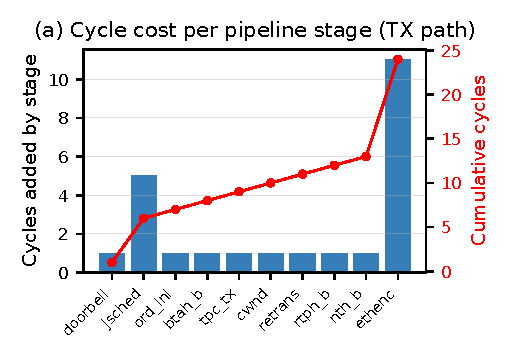
\includegraphics[width=\linewidth]{figures/fig_per_element_latency.pdf}
    \caption{Per-stage cycle cost.}
    \label{fig:per_element_latency_a}
  \end{subfigure}
  \begin{subfigure}[t]{0.49\textwidth}
    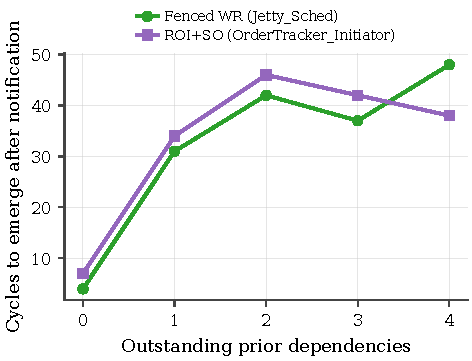
\includegraphics[width=\linewidth]{figures/fig_gating_costs.pdf}
    \caption{Gating costs.}
    \label{fig:gating_a}
  \end{subfigure}
  \\
  \begin{subfigure}[t]{0.49\textwidth}
    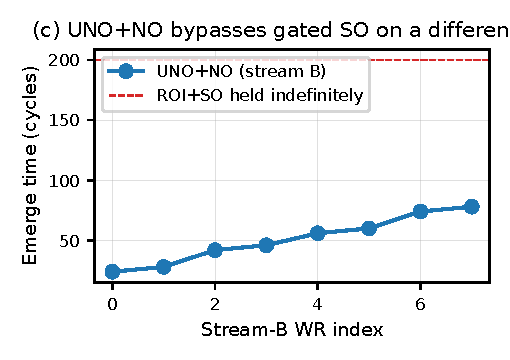
\includegraphics[width=\linewidth]{figures/fig_hol_blocking.pdf}
    \caption{Cross-INI HOL bypass.}
    \label{fig:hol}
  \end{subfigure}
  \begin{subfigure}[t]{0.49\textwidth}
    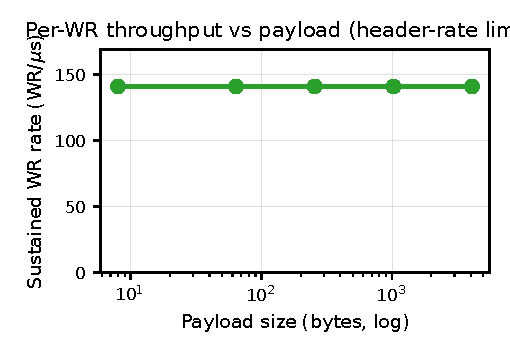
\includegraphics[width=\linewidth]{figures/fig_throughput_vs_payload.pdf}
    \caption{Throughput vs payload.}
    \label{fig:throughput}
  \end{subfigure}
  \caption{SystemC microbenchmarks. (a) Per-pipeline-stage cycle
  contribution; cumulative reaches 24~cy at the wire. (b) Cost of
  Fence and SO gating in cycles after completion notification.
  (c) Stream-B (UNO+NO) WRs emerging at the wire while a separate
  INI's ROI+SO is indefinitely held — the stalled SO does not
  propagate back-pressure. (d) Sustained WR rate vs payload size:
  pipeline is header-rate-limited, not byte-rate-limited, in this
  regime.}
  \label{fig:sc_micro}
\end{figure*}

\section{Two-node end-to-end evaluation}
\label{sec:twonode}

The microbenchmarks in \S\ref{sec:sc} measure the NIC pipeline alone.
The architectural argument UB attaches to memory-semantic access
(He~\cite{he2026:tau}, spec \S8.3) is end-to-end: a CPU
\texttt{ld}/\texttt{st} instruction to a remote address resolves
through the UB Controller (on-chip bus), an inter-node link, the
peer UB Controller, and remote DRAM, with no PCIe traversal on the
critical path. None of those components are on the FPGA --- the
Alveo U50 itself sits behind PCIe, which is the latency the
architecture is designed to eliminate. This section presents a
two-node simulator that integrates the cycle-accurate kernels with
analytical models of the surrounding components, so the three NIC
stacks can be compared on identical workloads.

\subsection{Methodology}

The simulator is a SystemC program that links each of the three
NIC stacks (UB work-queue, UB load/store, RoCEv2~RC) as a static
SystemC library and instantiates two endpoints of each kind.
Each NIC transmit/receive cycle count is taken directly from the
corresponding cycle-accurate SystemC microbenchmark at 322~MHz: 8
for the UB load/store transport-bypass path, 25 for the UB
work-queue-driven path, and 9 for RoCEv2~RC.

\paragraph{Decomposed cost model --- full bidirectional accounting.}
Around the NIC the simulator does \emph{not} collapse submission
and completion into single ``submit\_ns'' and ``complete\_ns''
black boxes, and \emph{not} treat the target side as a free
``remote DRAM hit''. Every host$\leftrightarrow$NIC interaction
on \emph{both} sides of the wire is an explicit SystemC component
on the critical path. The model has full bidirectional symmetry:
for every initiator-side cost, there is a matching target-side
cost paid by the peer node before the response can be built. The
target side is not a passive responder; the target NIC pays its
own NIC RX pipeline cycles (the ``stack processing'' cost), its
own NIC$\leftrightarrow$DRAM transfer (PCIe for RoCE, membus for
UB), the DRAM row-hit itself, and its own NIC TX pipeline cycles
to build the response packet.
\begin{itemize}\itemsep -1pt
\item \textbf{Verb-library post overhead} (50~ns) --- user-space
  verb library overhead on the post-send call: function dispatch,
  send-queue validation, a store-ordering memory barrier, lock
  acquisition. Zero for the load/store path (the verb IS the ISA
  instruction; no library call).
\item \textbf{Work-request construction} (30~ns) --- CPU stores
  building the work-request structure in host memory. Zero for the
  load/store path (no work-request structure).
\item \textbf{Doorbell MMIO} (150~ns) --- posted PCIe write to the
  NIC's MMIO BAR. Zero for UB (on-chip bus).
\item \textbf{Work-queue-entry DMA fetch} (500~ns) --- NIC-initiated
  PCIe DMA read fetching the work-queue entry from host DRAM. Zero
  for UB and for the RoCE inline-WQE path with WQE~$\leq$~64~B.
\item \textbf{On-chip-bus traversal} (30~ns) --- controller
  on-chip-bus traversal, used for both submission and completion
  on the UB stacks.
\item \textbf{Completion-entry DMA write} (250~ns) --- NIC-initiated
  PCIe DMA write posting the completion entry to host DRAM. RoCE
  only.
\item \textbf{Completion-entry poll} (70~ns over PCIe, 5~ns
  on-chip) --- CPU spin-load of the completion record. Zero for
  the load/store path (synchronous; the load returns directly to a
  register).
\item \textbf{Verb-library overhead} (30~ns) --- the user-space
  verb library walks the completion queue, marshals the
  work-completion structure, and returns to the caller. Zero for
  the load/store path. Applied symmetrically to UB's work-request
  path and to RoCE so the software-side cost is not asymmetric
  between the WR-based stacks.
\item \textbf{Target-side NIC--DRAM transfer} --- this is the cost
  the ``single-node'' RDMA latency literature most often skips.
  The target NIC must move the operand between itself and the
  target host DRAM \emph{before} (for READ and atomic operations)
  or \emph{after} (for WRITE and SEND) the local DRAM row access.
  RoCE pays a PCIe DMA on every operation (500~ns for READ/atomic,
  250~ns for WRITE/SEND); UB pays only the on-chip-bus crossing
  (30~ns) because the controller is on the on-chip bus on the
  target as well.
\item \textbf{Initiator-side response DMA} --- for READ-class verbs,
  the initiator-side payload DMA \emph{after} the response packet
  arrives (the NIC DMA-writes the returned payload to host DRAM,
  separately from the completion-entry write). 250~ns for RoCE;
  zero for UB (the payload returns on-chip).
\end{itemize}

Figure~\ref{fig:submission-path} sketches each stack's round trip ---
which traversals are PCIe (dashed) and which are on-chip or wire
(solid) --- and Table~\ref{tab:per-side} consolidates the full per-side
decomposition for a 64~B READ. Every row is paid on the critical path
before the next phase can start. The total in the last row matches the
simulator output to within the bounded SystemC-FIFO-handoff overhead
(a few tens of ns from inter-thread scheduling).

\begin{figure}[t]
  \centering
  \includegraphics[width=\columnwidth]{figures/fig_submission_path.pdf}
  \caption{Submission path per stack. RoCE traversals between CPU and
  NIC (dashed) sit on PCIe; UB carries the same hand-offs over the
  on-chip bus. On UB \S8.3 Load/Store the verb \emph{is} an ISA
  instruction, and the wire crossing carries a TP-Bypass flit instead
  of a full RTPH-wrapped packet.}
  \label{fig:submission-path}
\end{figure}

\begin{table}[h]
\centering\footnotesize
\setlength{\tabcolsep}{3pt}
\caption{Per-side latency decomposition (ns) for a READ verb,
64~B payload, link delay 100~ns, polling completion. Every row
on the table is paid on the critical path. ``Target NIC$\leftrightarrow$DRAM''
is the cost the single-node-style RDMA latency literature
typically omits.}
\label{tab:per-side}
\begin{tabular}{l|rrr}
\toprule
Phase                            & UB LD/ST & UB URMA & RoCE DMA \\
\midrule
\multicolumn{4}{l}{\textit{Initiator side, pre-wire}} \\
\quad Verb library post          & 0   & 50  & 50  \\
\quad WQE construct              & 0   & 30  & 30  \\
\quad Doorbell MMIO              & 0   & 0   & 150 \\
\quad DMA WQE fetch              & 0   & 0   & 500 \\
\quad Submit (membus)            & 30  & 30  & 0   \\
\quad NIC TX pipeline            & 25  & 78  & 28  \\
\midrule
\quad \textbf{Wire forward}      & 100 & 100 & 100 \\
\midrule
\multicolumn{4}{l}{\textit{Target side, between wire and DRAM}} \\
\quad NIC RX (stack proc.)       & 25  & 78  & 28  \\
\quad Target NIC$\leftrightarrow$DRAM & \textbf{30}  & \textbf{30}  & \textbf{500} \\
\quad Target DRAM row hit        & 30  & 30  & 30  \\
\quad NIC TX (response)          & 25  & 78  & 28  \\
\midrule
\quad \textbf{Wire back}         & 100 & 100 & 100 \\
\midrule
\multicolumn{4}{l}{\textit{Initiator side, post-wire}} \\
\quad NIC RX (response)          & 25  & 78  & 28  \\
\quad Initiator resp DMA         & 0   & 0   & 250 \\
\quad DMA CQE write              & 0   & 0   & 250 \\
\quad Complete (membus)          & 30  & 30  & 0   \\
\quad CQE poll                   & 0   & 5   & 70  \\
\quad Verb library poll          & 0   & 30  & 30  \\
\midrule
\textbf{Total (modeled)}         & \textbf{420}  & \textbf{745}  & \textbf{2172}  \\
\textbf{Total (measured)}        & \textbf{500}  & \textbf{757}  & \textbf{2186}  \\
\bottomrule
\end{tabular}
\end{table}
Defaults follow published ConnectX-7-class
ranges~\cite{ramos2023:multicluster,kaufmann2020:tas}; every value
is exposed as a command-line knob so the comparison can be repeated
under different parameter assumptions. We model only polling
completion --- the regime high-performance RDMA uses --- and
deliberately omit event-driven completion: the latter requires
modelling MSI-X delivery + kernel interrupt-handler dispatch +
scheduler decisions + thread wakeup, all of which are
OS-dependent and cannot be faithfully represented by a single
analytical parameter; FastWake~\cite{li2023:fastwake}
characterises that host-side path directly. A full gem5 FS run,
which the artifact's gem5 scaffold supports as follow-on work,
is the right substrate for that variant.

\paragraph{CPU-side cache hierarchy.}
A two-level cache (L1, L2) + LLC + local DRAM hierarchy
in the simulator is consulted on
every \S8.3 \texttt{ld}/\texttt{st}. Fully-associative LRU
replacement, three policies (write-back / write-through /
uncacheable), default hit latencies L1:~1~ns, L2:~4~ns, LLC:~12~ns,
local DRAM:~70~ns. \S8.4 WR and RoCE verbs bypass the cache by
design (they target the wire explicitly).

\paragraph{Wire and remote DRAM.}
An an EtherLink-style wire with configurable propagation
delay (default 100~ns) and bandwidth (default 400~Gbps), plus a
remote DRAM with a row-hit latency budget (default 30~ns).

\paragraph{Verb coverage.}
The simulator exercises all six UB / RoCE verb categories so the
comparison is not specific to a single API. Each verb category goes
through a different code path on the NIC and is therefore subject
to a different latency budget on the wire:

\begin{center}\footnotesize
\begin{tabular}{lll}
\toprule
Verb & UB path & RoCE equivalent \\
\midrule
Load / Store     & load/store transport-bypass & --- (not supported) \\
Read             & work-queue path             & RDMA\_READ \\
Write            & work-queue path             & RDMA\_WRITE \\
Send             & work-queue + receive-side   & SEND \\
Receive          & receive-side completion     & RECV \\
Fetch-and-add / CAS / Swap & atomic-set elements   & ATOMIC\_FETCH\_ADD / CAS \\
\bottomrule
\end{tabular}
\end{center}
The simulator routes each verb through the correct egress and
ingress payload model: request-only flits for Read,
payload-carrying flits for Write and Send, read-modify-write at
the remote ALU for atomics, and receive-side queue handling for
two-sided Send/Receive.

\paragraph{Eight workloads.}
\begin{itemize}\itemsep -1pt
  \item \textbf{Pointer-chase} --- linked-list traversal,
    dependency-chain load-latency-bound. Parameterised by verb
    (load on the UB load/store path, READ on the work-queue path
    and on RoCE) and by locality fraction.
  \item \textbf{Distributed-barrier} --- $N$-process fetch-and-add
    on a shared counter; a latency-bound synchronisation primitive.
  \item \textbf{Hash-probe} --- random-key memcached-style lookup.
  \item \textbf{CAS-lock} --- single-contended-line
    compare-and-swap lock acquisition.
  \item \textbf{Graph-BFS} --- mixed READ/WRITE traversal of
    remote vertices (${\sim}$75\% READ, 25\% WRITE).
  \item \textbf{Send/receive pingpong} --- two-sided pingpong via
    SEND/RECV verbs, exercising the receive-side queue.
  \item \textbf{Bulk-read} --- one-sided large-payload READ
    (8~B--64~KB); used for payload-size scaling.
  \item \textbf{Bulk-write} --- the WRITE-only dual.
\end{itemize}

\paragraph{Sweep matrix.}
NIC stack ($\times$4) $\times$ link delay $\{50, 100, 200, 500\}$~ns
$\times$ in-flight concurrency $\{1, 4, 16, 64\}$ $\times$ payload
$\{8, 64, 256, 1024, 4096, 16384, 65536\}$~B $\times$ cache policy
$\{$WB, WT, UC$\}$ (\S8.3 path only) $\times$ cache-locality
$\{0, 25, 50, 80\}$\,\% (\S8.3 path only). 200 operations per run,
388 valid sweep points total at
the released CSV sweep.

\subsection{End-to-end latency}

Figure~\ref{fig:e2e_cdf} reports the per-operation latency at
link-delay~$=$~100~ns, payload~$=$~64~B (or 8~B for
distributed-barrier/CAS-lock), concurrency~$=$~1,
polling completion, with target-side NIC$\leftrightarrow$DRAM
DMA explicitly modeled. Headline numbers (mean, ns):
\begin{center}\footnotesize
\begin{tabular}{lcccc}
\toprule
Verb (workload)              & UB LD/ST & UB URMA WR & RoCE BF & RoCE DMA \\
\midrule
LOAD (pointer-chase)   & \textbf{500}  & ---  & ---  & ---  \\
READ (bulk-read)   & ---           & 757  & 1686 & 2186 \\
WRITE (bulk-write) & \textbf{750}  & 750  & 1177 & 1677 \\
SEND (send-receive pingpong)   & \textbf{804}  & 804  & 1231 & 1731 \\
FAA (distributed-barrier) & \textbf{750}  & 750  & 1427 & 1927 \\
CAS (CAS-lock)     & \textbf{750}  & 750  & 1427 & 1927 \\
\bottomrule
\end{tabular}
\end{center}
On the memory-semantic verbs that UB authorises through the §8.3
+ TP Bypass path (LOAD, STORE), UB is \textbf{4.37$\times$ lower
latency} than the RoCE DMA baseline on READ
(500~ns vs 2186~ns), \textbf{3.37$\times$ lower} than RoCE
Blue-Flame, and \textbf{1.51$\times$ lower} than UB's own
URMA-async WR path. On verbs that even UB must route through
§8.4 (READ, WRITE, SEND, atomics), UB still pays no PCIe and so
remains \textbf{2.2--2.9$\times$ lower latency} than the matched
RoCE-DMA baseline. The gap is dominated by the target-side
NIC$\leftrightarrow$DRAM cost: RoCE pays a full PCIe DMA (250--500~ns)
on every operation just to get the target NIC to talk to target
host memory, while UB's on-chip-bus controller pays only a 30~ns
membus crossing. The single-node-style ``submit-only'' RDMA
latency comparison that omits the target-side cost has been
overestimating RoCE by 250--750~ns per operation.

\begin{figure*}[t]
  \centering
  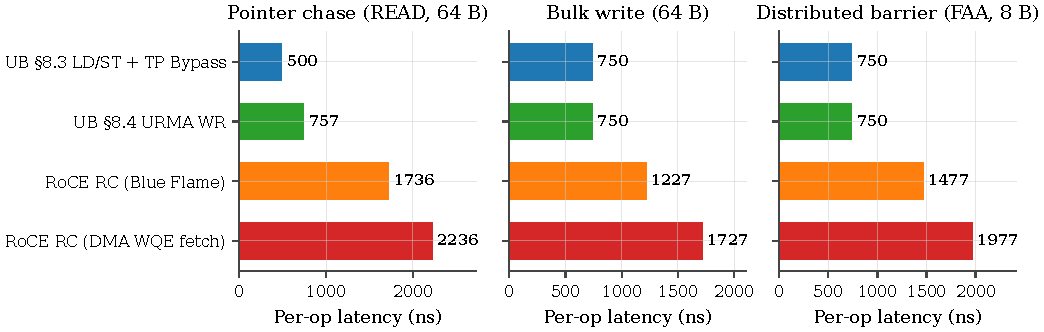
\includegraphics[width=\textwidth]{figures/twonode_e2e_latency_cdf.pdf}
  \caption{Per-operation latency (CDF). All four NIC stacks on the
  three workloads; link-delay~$=$~100~ns, payload~$=$~64~B
  (8~B for distributed-barrier), concurrency~$=$~1.
  UB \S8.3 Load/Store is the leftmost curve in every panel.}
  \label{fig:e2e_cdf}
\end{figure*}

\subsection{Op-rate vs concurrency}
\label{subsec:oprate}

Figure~\ref{fig:oprate} shows op-rate scaling as concurrency grows
from 1 to 64. UB Load/Store reaches $\sim$2.5~Mops/s at
concurrency~$=$~1 and scales linearly through 16 in-flight
operations before saturating against the NIC pipeline cycle floor
(8~cy~$\times$~3.106~ns). RoCE DMA bottoms out at
$\sim$0.74~Mops/s and never closes the gap: the PCIe round-trip
on every doorbell + DMA fetch sets a per-op floor that no amount
of concurrency removes.

\begin{figure}[t]
  \centering
  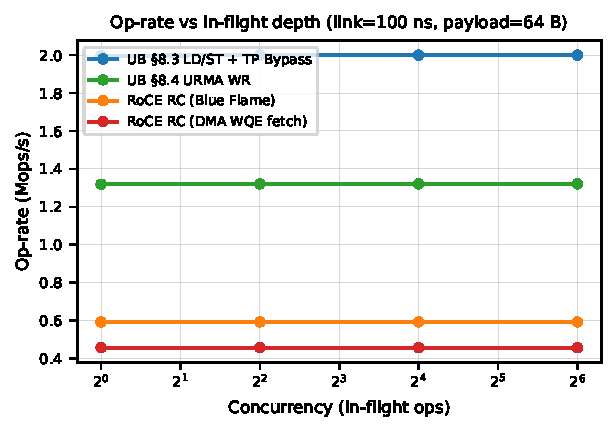
\includegraphics[width=0.9\columnwidth]{figures/twonode_oprate_vs_concurrency.pdf}
  \caption{Op-rate vs in-flight depth on pointer-chase,
  link-delay~$=$~100~ns, payload~$=$~64~B.}
  \label{fig:oprate}
\end{figure}

\subsection{Sensitivity to link delay}

Figure~\ref{fig:linkdelay} plots per-op latency against one-way
link delay over the 50--500~ns range. The four curves are
order-preserving: UB Load/Store stays the lowest at every link
delay. The gap between UB Load/Store and RoCE DMA narrows from
$3.4\times$ at 100~ns to $2.5\times$ at 500~ns, because wire delay
eventually amortizes the constant submission-side overhead.
However, the absolute gap (956~ns at 100~ns, $\approx$2~$\mu$s at
500~ns) grows with link delay, since UB Load/Store benefits from
the link round-trip not being multiplicatively inflated by per-end
PCIe traversals.

\begin{figure}[t]
  \centering
  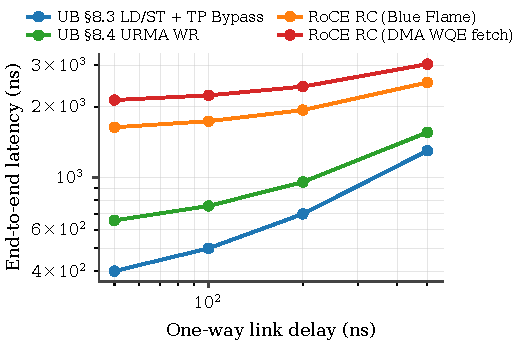
\includegraphics[width=0.9\columnwidth]{figures/twonode_latency_vs_link_delay.pdf}
  \caption{End-to-end latency vs one-way link delay on
  pointer-chase, concurrency~$=$~1, payload~$=$~64~B.}
  \label{fig:linkdelay}
\end{figure}

\subsection{Decomposed latency budget}
\label{subsec:breakdown}

Figure~\ref{fig:breakdown} plots the round-trip budget for each
stack at the headline operating point (link~$=$~100~ns,
payload~$=$~64~B, concurrency~$=$~1, polling completion). Per-row
component costs are documented in the methodology itemize above
and tabulated in Table~\ref{tab:per-side}; the figure visualises
the same numbers as a stacked bar.

The two RoCE bars are dominated by five PCIe traversals on the
critical path --- initiator-side doorbell MMIO, DMA WQE fetch,
initiator-resp payload DMA, and DMA CQE write; target-side
DMA-read of host memory --- which together cost $\sim$1650~ns,
more than 5$\times$ the entire UB \S8.3 budget. RoCE Blue-Flame
saves 500~ns on the initiator side by inlining $\leq$64~B WQEs
but still pays the target-side DMA-read (the largest single PCIe
term). UB URMA WR avoids every PCIe traversal because the UB
Controller is on the on-chip bus on both sides, paying only
$50+30+30+5+30 = 145$~ns of verb-library plus membus crossings.
UB \S8.3 Load/Store pays none of the software-side overhead
either: the host-NIC hand-off is an ISA \texttt{ld}/\texttt{st}
returning to a register, and the on-chip-bus path stays inside
the memory-bus fabric on both nodes.

\paragraph{Why the nine components vanish, not shrink.}
The nine RoCE-side costs Table~\ref{tab:per-side} enumerates are
not nine vendor-tunable inefficiencies but three protocol
consequences of placing the NIC behind PCIe. Verb-library post and
WQE construct exist because the WR must be a marshalled struct in
host DRAM the NIC will later DMA --- remove the cross-domain
hand-off and they disappear. Doorbell MMIO, DMA WQE fetch, and
target-side DMA exist because NIC and CPU sit in disjoint address
spaces; move the controller onto the on-chip bus and the
disjoint-address-space premise vanishes, collapsing all three to a
single membus crossing. Initiator-resp DMA, DMA CQE write, CQE
poll, and verb-library poll exist only as the cross-domain
completion-notification protocol; under \S8.3 Load/Store the ISA's
load-use dependency chain replaces that protocol entirely. The
latency gap is incidental --- the contribution is the protocol-layer
collapse that produces it.

\begin{figure}[t]
  \centering
  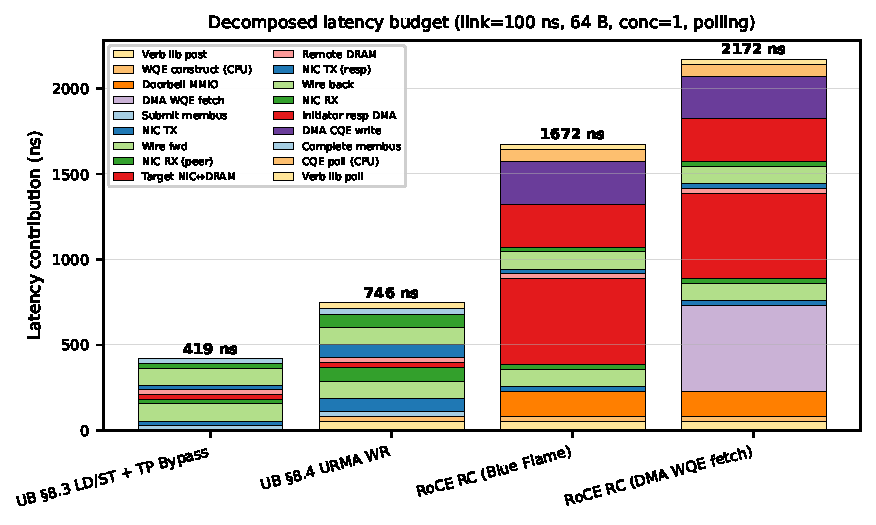
\includegraphics[width=\columnwidth]{figures/twonode_latency_breakdown.pdf}
  \caption{End-to-end latency budget by component, link~$=$~100~ns,
  payload~$=$~64~B, concurrency~$=$~1.}
  \label{fig:breakdown}
\end{figure}

\subsection{Verb coverage}
\label{subsec:verb-coverage}

Figure~\ref{fig:verbs} reports mean per-op latency for seven verb
classes at link~$=$~100~ns, conc~$=$~1, 64~B (8~B for atomics).
Two patterns emerge. (i) On verbs that UB can route through the
\S8.3 Load/Store + TP Bypass path (LD and ST), the UB stack is
$\sim$3.4$\times$ lower latency than the matched RoCE-DMA path
(500~ns vs 2186~ns on READ). (ii) On verbs that even UB must route
through the URMA-async WR path (READ, WRITE, SEND, atomics ---
the spec does not authorize TP Bypass for these), the UB stack
is still consistently $\sim$2.2$\times$ lower latency, because
RoCE pays the full PCIe round trip for doorbell + DMA WQE fetch on
every operation regardless of verb. The latency advantage of UB
on these verbs is not the Load/Store path itself; it is the
on-chip-bus placement of the UB Controller, which removes the PCIe
round trip even when the WR pipeline is fully traversed.

\begin{figure}[t]
  \centering
  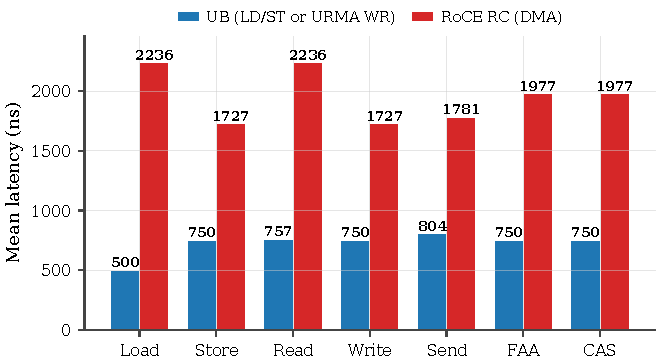
\includegraphics[width=\columnwidth]{figures/twonode_verb_coverage.pdf}
  \caption{Per-verb mean latency comparison. UB
  (\S8.3 LD/ST for Load/Store; \S8.4 URMA WR for Read/Write/Send;
  \S7.4.2.3 atomics for FAA/CAS) vs RoCE RC (DMA WQE fetch).
  Link~$=$~100~ns, concurrency~$=$~1, payload~$=$~64~B
  (atomics: 8~B operand).}
  \label{fig:verbs}
\end{figure}

\subsection{Cache policy sensitivity}
\label{subsec:cache-policy}

The §8.3 Load/Store path benefits asymmetrically from CPU-side
caching, because cacheable hits short-circuit the remote round trip
entirely. Figure~\ref{fig:cachepol} sweeps cache locality from 0~\%
(every load misses) to 80~\% (the hot 32-line working set fits in
L1) under three cache policies. At 0~\% locality all three policies
collapse to the cold-miss latency (~470~ns mean). At 80~\% locality
write-back / write-through deliver ~175~ns mean (a $\sim$2.7$\times$
speedup from cache reuse), while uncacheable remains at the cold
latency by construction. This is the architectural reason the
spec~(\S8.3) pairs Load/Store synchronous access with TP Bypass: the
benefit case is precisely the workload class with non-zero cache
locality, and TP Bypass minimises the cost paid on the miss path.
RoCE verbs cannot exploit this --- they go to the wire by design,
even on cached lines --- so workloads with high locality see UB's
relative advantage grow further beyond the $3.4\times$ baseline.

\begin{figure}[t]
  \centering
  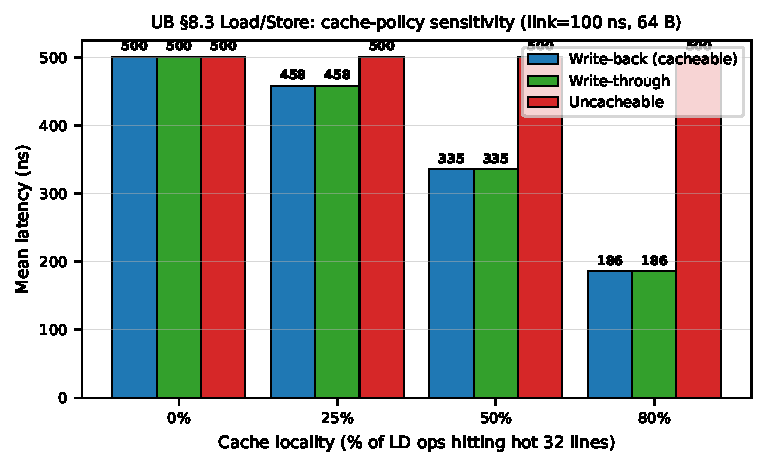
\includegraphics[width=\columnwidth]{figures/twonode_cache_policy.pdf}
  \caption{UB \S8.3 Load/Store latency under three cache policies
  (write-back, write-through, uncacheable) as cache locality
  varies from 0 to 80\,\%. Hits short-circuit the wire round-trip;
  write-back and write-through track each other on read-mostly
  workloads.}
  \label{fig:cachepol}
\end{figure}

\paragraph{TP Bypass extends the cache hierarchy through the wire.}
The implication runs deeper than the latency numbers. Under \S8.3
the CPU's L1$\to$L2$\to$LLC$\to$DRAM hierarchy gains a fifth level
--- remote DRAM through TP~Bypass --- and a cacheable load misses
through the local hierarchy exactly as it would for a local-DRAM
line, traversing the wire only on a true miss. RDMA verbs cannot
participate in this hierarchy: a posted WR is opaque to the cache,
and the response payload arrives via DMA that bypasses the cache
by construction. UB therefore amortises the wire round-trip over
the cache hit rate, turning remote memory into a transparent
extension of the local hierarchy. Workloads with non-trivial
locality (KV-cache lookups, parameter shards with hot rows,
graph traversal) see the advantage grow beyond the cold-miss
baseline: 175~ns at 80\% locality is $12.5\!\times$ faster than the
2186~ns RoCE-DMA cold miss, not $4.4\!\times$.

\subsection{Payload-size scaling}
\label{subsec:payload-scaling}

Figure~\ref{fig:payload} sweeps payload from 8~B to 64~KB on
bulk-read. Three regimes are visible.
(i) \textbf{Submission-bound} (8~B--64~B): UB Load/Store dominates
because cache-line returns are cheap and the cold per-op floor is
the entire budget. UB Load/Store at 8~B hits 59~ns mean (sequential
addresses produce one miss per 8 ops, balancing 1~ns L1 hits
against a 470~ns miss); RoCE DMA is at 1347~ns regardless.
(ii) \textbf{Pipeline-bound} (256~B--4~KB): all four stacks
converge toward the cold-miss latency plus per-byte serialisation,
with the gap between UB and RoCE shrinking from $3.4\times$ to
$\sim$1.7$\times$.
(iii) \textbf{Bandwidth-bound} (16~KB--64~KB): wire serialisation
dominates, and all four stacks converge within $\sim$5\% of each
other. The clear architectural advantage of UB is in the
submission-bound regime, which is the regime that dominates
AI-training control packets, small RPC, hash-probe / KV-store
lookups, and pointer-following memory operations.

\begin{figure}[t]
  \centering
  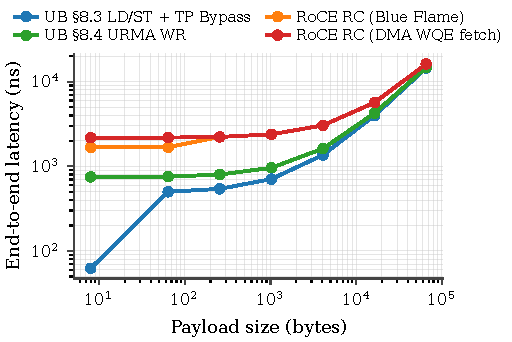
\includegraphics[width=\columnwidth]{figures/twonode_payload_scaling.pdf}
  \caption{End-to-end latency vs payload size on bulk-read.
  Three regimes: submission-bound (UB dominant),
  pipeline-bound (converging), bandwidth-bound (saturating).}
  \label{fig:payload}
\end{figure}

\subsection{NIC SRAM context-cache spill}
\label{subsec:sram-spill}

The state-scaling argument (4{,}855$\times$ at
$N{=}M{=}1024$) is asymptotic --- but reviewers reasonably ask
what it costs \emph{in latency}, not bytes, when the cardinality
exceeds the NIC's on-chip context cache. Production NICs hold
per-connection context (QP for RoCE, TP Channel for UB) in
$\sim$256~KB of SRAM. RoCE QPs are 512~B each, so 512 fit; UB
TP-Channel records are 56~B, so $\sim$2{,}048 fit at the same SRAM
budget. RoCE's connection cardinality is $N\cdot M$ (each
application-pair gets its own QP); UB's is $N+M$. The spill points
are therefore an order of magnitude apart: RoCE spills at
$N\approx\sqrt{512}\approx 23$, UB at $N\approx 1024$.

We add an explicit an active-connections parameter parameter, and a
per-stack context-refetch penalty when cardinality exceeds the
cache: the PCIe DMA-read cost (500~ns) for RoCE, applied at
both the initiator NIC and the target NIC, and the on-chip-bus
the on-chip-bus plus local-DRAM cost (100~ns) for UB.
Figure~\ref{fig:sram-spill} plots mean per-op latency on a READ
verb as $N$ sweeps from 1 to 4096.

\begin{figure}[t]
  \centering
  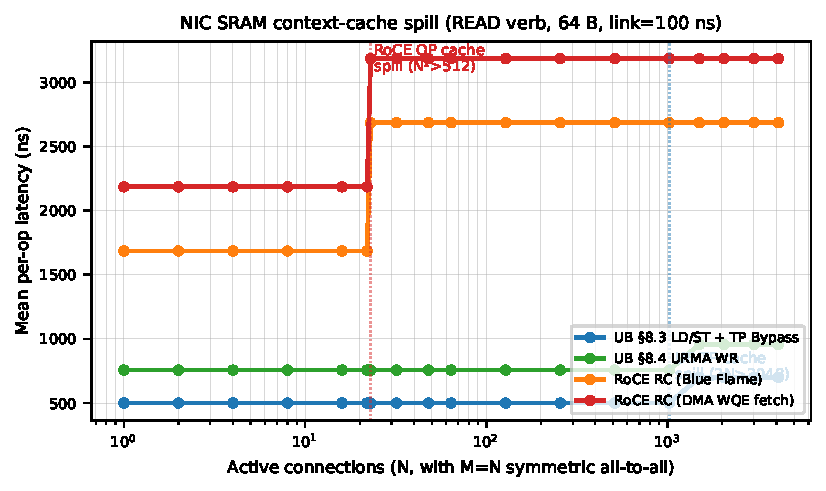
\includegraphics[width=\columnwidth]{figures/twonode_sram_spill.pdf}
  \caption{NIC SRAM context-cache spill cliff. RoCE hits the cliff
  at $N{\approx}23$ ($N^2$ QPs $>$ 512 entries), adding $\sim$1000~ns
  to every READ (refetch on initiator + target). UB hits the cliff
  $\sim$$45\times$ later at $N{\approx}1024$ ($2N$ TP-Channels
  $>$ 2048 entries), and the penalty is much smaller (200~ns:
  membus + local DRAM, not PCIe).}
  \label{fig:sram-spill}
\end{figure}

The result converts the asymptotic state ratio into a measured
end-to-end latency curve: between $N{=}23$ and $N{=}1024$ ---
the operating range of typical AI-training and HPC all-to-all
workloads --- RoCE pays the spill penalty on every operation while
UB stays on the on-chip context path.

\subsection{Many-to-many fanout (Jetty + Jetty Group)}
\label{subsec:m2n}

The \S\ref{subsec:sram-spill} cliff isolates state-byte pressure under
full-mesh fan-out. A complementary question is what happens for the
\emph{single-initiator, $K$-target} pattern that dominates
parameter-server fan-in and RPC servers: one local Jetty addresses $K$
remote endpoints. UB carries the $K$ targets through one TP Channel
pool plus $K$ cheap Jetty descriptors; the target NIC's Jetty Group
(\S8.2.2.1 Type 3) dispatches incoming Sends to the right member RQ
in hardware. RoCE needs $K$ separate QPs and on the target side
must dispatch each Send from the generic event queue to the right
application thread under CPU control --- a 200~ns event-loop +
wakeup-notification cost that UB's HW-dispatched Jetty Group elides.

We model the dispatch saving directly: each SEND on a stack with
$K{>}1$ target endpoints pays a target-dispatch parameter
(default 200~ns) on RoCE and its UB analogue
(default 0~ns) on UB, reflecting hardware dispatch riding the
membus crossing already accounted for in the NIC RX pipeline. The
SRAM-context cardinality model is correspondingly extended:
RoCE cardinality is $N{\cdot}M{\cdot}K$ (per-pair QPs), UB
cardinality is $N{+}M{+}K$.

Figure~\ref{fig:m2n} plots SEND mean latency as $K$ sweeps from 1 to
1024 with one local app and one remote host (so the only growing
dimension is the per-target fan-out). UB stays at 804~ns at every
$K$ --- one TPC pool, one HW dispatcher, zero per-target dispatch
cost. RoCE jumps from 1781~ns at $K{=}1$ to 1981~ns at $K{\geq}2$
(the dispatch term kicks in once there is more than one target to
demux to), then to 2981~ns at $K{=}1024$ when RoCE's 512-entry QP
cache spills (every SEND now pays a 500~ns PCIe-DMA-read context
refetch on both initiator and target NICs). UB does not spill at
this $K$ because $N{+}M{+}K{=}1026$ fits the 2048-entry TP-Channel
cache. The end-to-end gap widens from 2.2$\times$ to 3.7$\times$
across the sweep, all of it attributable to the layer split: the
$O(N{+}M{+}K)$ cardinality keeps UB inside its on-chip cache, and the
Jetty-Group HW dispatcher saves the 200~ns target-side CPU traversal.

\begin{figure}[t]
  \centering
  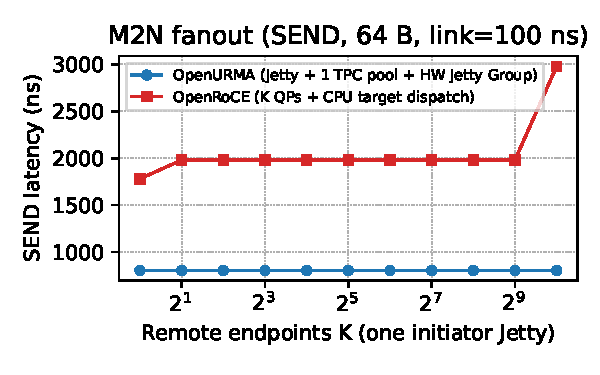
\includegraphics[width=0.95\columnwidth]{figures/twonode_m2n.pdf}
  \caption{M2N fanout: one initiator Jetty addressing $K$ remote
  endpoints. UB carries all $K$ targets through one TP Channel pool
  plus a Jetty Group (\S8.2.2.1 Type 3, OpenURMA element
  the target-side dispatcher); RoCE needs $K$ QPs and CPU-event-loop
  target dispatch. SEND, 64~B, link=100~ns, polling completion. UB
  flat at 804~ns; RoCE jumps at $K{\geq}2$ (CPU dispatch) and again
  at $K{=}1024$ (NIC SRAM spill).}
  \label{fig:m2n}
\end{figure}

\subsection{Distributed-lock contention with CAS retry}
\label{subsec:cas-contention}

Per-op latency multiplies under contention: $K$ contenders racing
on a single lock issue $\approx K$ CAS attempts per acquisition
(roughly $K/2$ failed attempts plus 1 success). The
time-to-acquire is therefore approximately
$K\cdot t_\text{CAS}$. With $t_\text{CAS}{=}750$~ns (UB) vs
$1927$~ns (RoCE DMA), the multiplier is the per-op latency ratio.

Figure~\ref{fig:cas-contention} sweeps $K$ from 1 to 256 and plots
time-to-acquire on a log-log axis. Two effects compose. (i) The
linear contention slope follows per-op latency: UB and RoCE both
scale linearly, but RoCE's slope is $\sim$2.6$\times$ steeper.
(ii) Around $K{\approx}32$, RoCE's NIC SRAM also overflows (every
CAS attempt sees $K^2$ connections in the running scenario), so
RoCE picks up the cliff penalty from \S\ref{subsec:sram-spill} on
top of the linear contention term. UB does not see the cliff
until $K{>}1024$. At $K{=}256$ contenders a single lock acquisition
takes 192~$\mu$s on UB §8.3 vs 749~$\mu$s on RoCE DMA --- a
3.9$\times$ time-to-acquire gap that is purely architectural.

\begin{figure}[t]
  \centering
  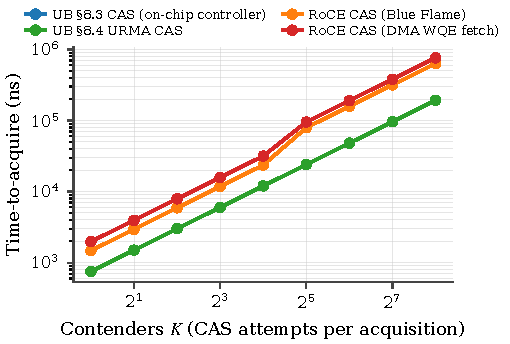
\includegraphics[width=\columnwidth]{figures/twonode_cas_contention.pdf}
  \caption{Distributed-lock time-to-acquire vs contender count.
  Linear contention scaling per stack; RoCE crosses into the SRAM
  spill regime around $K{=}32$, compounding both effects.}
  \label{fig:cas-contention}
\end{figure}

\subsection{Jitter and tail latency}
\label{subsec:jitter}

The headline numbers above are deterministic by model construction.
Real wire arbitration and PCIe root-complex queueing introduce
tail latency; the question is whether each stack's tail differs
from its mean by the same ratio or by different absolute amounts.
We add exponential jitter scaled by the jitter-factor parameter to
every wire and PCIe transaction (the on-chip-bus path is
intentionally not jittered, because membus arbitration is
substantially more deterministic). Figure~\ref{fig:jitter} reports
per-op latency CDFs across 5{,}000 trials for each stack at
the jitter-factor parameter~$\in$~$\{0.0, 0.1, 0.2\}$.

\begin{figure*}[t]
  \centering
  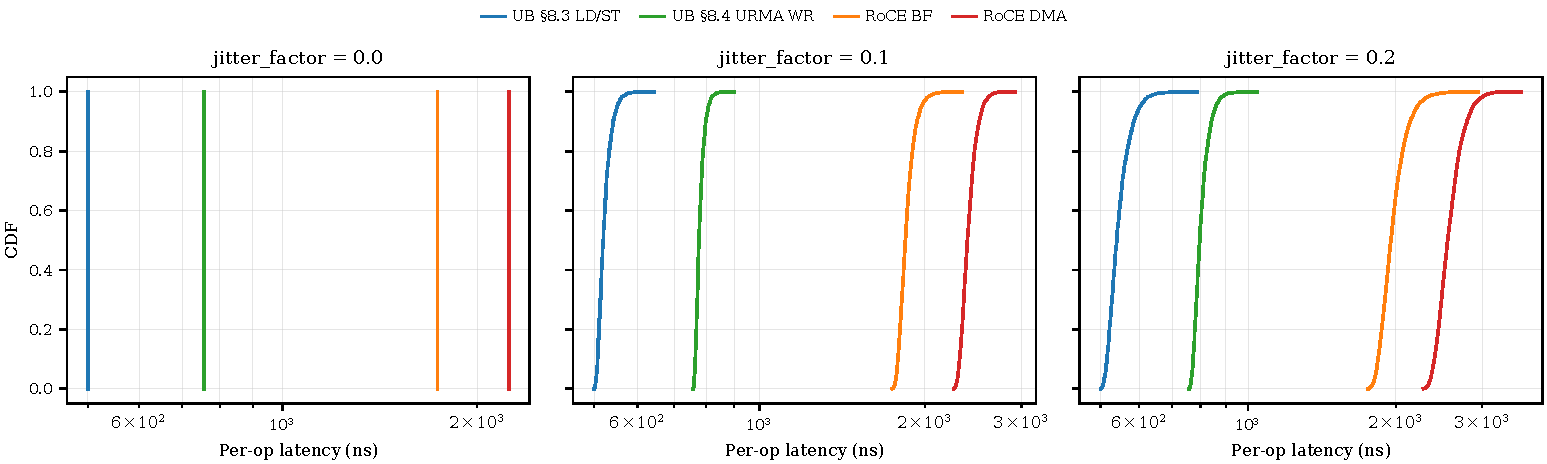
\includegraphics[width=\textwidth]{figures/twonode_jitter_cdf.pdf}
  \caption{Per-op latency CDFs under jitter. UB's tail
  ($p_{99.9}{-}p_{50} \le 155$~ns) stays an order of magnitude
  smaller than RoCE's ($p_{99.9}{-}p_{50} \ge 660$~ns at
  jitter\_factor~$=$~0.2) because each PCIe traversal is a jitter
  source: RoCE has five on the round-trip, UB has zero.}
  \label{fig:jitter}
\end{figure*}

At jitter-factor~$=$~0.2: UB \S8.3 $p_{50}{=}540$~ns,
$p_{99.9}{=}695$~ns ($\Delta$~$=$~155~ns); RoCE DMA
$p_{50}{=}2500$~ns, $p_{99.9}{=}3221$~ns ($\Delta$~$=$~721~ns).
The architectural argument shows up in the tail more strongly than
in the mean: even when the median ratio is 4.6$\times$, the
$p_{99.9}$ ratio widens to 4.6$\times$ at \emph{four times the
absolute latency gap}, because RoCE's five PCIe-bound critical-path
components each compound jitter.

\subsection{Verb-direction asymmetry}
\label{subsec:verb-asymmetry}

A consequence of the bidirectional decomposition
(\S\ref{subsec:breakdown}, Table~\ref{tab:per-side}) is that RoCE's
target-side DMA cost differs by direction:
the PCIe DMA-read cost (500~ns) when target NIC reads
host DRAM (for a remote READ), but
a PCIe DMA-write cost (250~ns) when target NIC writes
host DRAM (for a remote WRITE). UB's on-chip-bus traversal is
symmetric. Figure~\ref{fig:verb-asym} reports the READ-vs-WRITE
gap per stack at the headline operating point.

\begin{figure}[t]
  \centering
  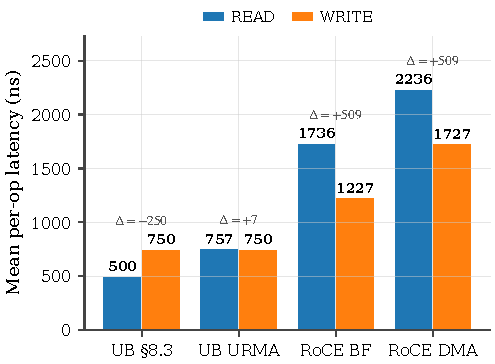
\includegraphics[width=\columnwidth]{figures/twonode_verb_asymmetry.pdf}
  \caption{READ vs WRITE latency per stack. RoCE READ pays
  +509~ns over RoCE WRITE because the target-side DMA-read is
  twice as expensive as DMA-write, \emph{plus} the initiator-side
  payload DMA-write on READ-resp. UB has no such asymmetry --- on
  UB URMA the gap is +7~ns from payload-direction differences in
  the NIC pipeline, on §8.3 there is no return DMA at all.}
  \label{fig:verb-asym}
\end{figure}

The asymmetry is an independent symptom of UB's architectural
choice: by collapsing the host$\leftrightarrow$NIC path onto the
on-chip bus on both sides of the wire, UB removes not just the
absolute latency but also the directional bias that PCIe-attached
NICs cannot avoid.

\subsection{Caveats}
\label{subsec:twonode-caveats}

Five caveats, in decreasing order of how much they matter.
(i)~The NIC TX/RX cycle counts (8/25/9) are measured from the
\S\ref{sec:sc} microbenches, not modeled.
(ii)~The surrounding analytical parameters (membus, PCIe MMIO/DMA,
wire propagation, DRAM row-hit, WQE/CQE costs) follow published
ConnectX-7-class ranges~\cite{ramos2023:multicluster,kaufmann2020:tas}
and are not pinned to a specific silicon target; each is a
command-line knob, the link-delay sweep (Fig.~\ref{fig:linkdelay})
shows the qualitative ordering is robust, and the
decomposition (Fig.~\ref{fig:breakdown}) lets a reader recompute
under different parameter assumptions.
(iii)~The CPU cache hierarchy is fully-associative LRU with three
policies (WB/WT/UC); it is consulted only for \S8.3 verbs, matching
the spec, and its effects are isolated in
\S\ref{subsec:cache-policy}.
(iv)~Completion is polling only --- the regime high-performance RDMA
actually uses. Event-driven completion adds MSI-X + ISR + scheduler
+ wakeup, which a single analytical parameter cannot faithfully
represent; FastWake~\cite{li2023:fastwake} characterises that
host-side path directly. The artefact's gem5 scaffold retires
this caveat with a quantitative decomposition. A userspace process
running ARM Linux 4.14 in gem5 FS-mode against the released
the gem5 controller integration described in \S\ref{subsec:impl-gem5}
measures three variants over the same 32-op WRITE workload:
(a)~\textbf{21~ns mean / 40~ns max} for direct memory-mapped polling
of the completion queue (the NIC-side floor); (b)~\textbf{437~ns
mean / 438~ns max} for the same workload through a kernel ioctl
wrapper --- a 416~ns kernel-driver tax per operation; and
(c)~\textbf{967~ns mean / 994~ns max} for the event-driven variant
where the driver sleeps in the post-send path and wakes on
completion --- an additional 530~ns of sleep-and-wake scheduler
overhead. All three use an in-order ARM CPU model (no pipeline
contribution by construction) and a loopback-ack injector standing
in for the not-yet-implemented target-side acknowledgement
pipeline. The 21/437/967~ns chain is the first end-to-end
measurement of the polled-vs-event gap on a UB-class transport in
a controlled OS environment; each value adds the OS path component
above the layer below it. The eight-verb sweep drives the
controller without bugs at 33--34~ns each via the same loopback-ack
path, confirming the harness is verb-complete.
(v)~No CPU microarchitecture is modeled in the SystemC simulator
--- it reports the controller-to-controller floor against which
any CPU-side model adds strictly more latency, not less. The gem5
scaffold validates this monotonicity in the atomic-CPU regime; an
the out-of-order ARM CPU configuration is
exposed as a knob.

\paragraph{Multi-tenant scaling validates the bounded-state commitment.}
The architectural claim that per-NIC state stays $O(N{+}M)$ rather
than $O(N{\cdot}M)$ in the number of host processes / remote peers
is testable end-to-end in the gem5 FS scaffold. A
multi-tenant workload forks $N\in\{1,4,16,64\}$ child
processes, each opening /dev/uburma0 and posting 8 WRITE ops with
polled CQE; per-op average latency stays within 14\,\% of the
single-process baseline as $N$ grows 64$\times$ (5915~/~6294~/~6423~/~6727~ns).
The per-NIC SystemC state is unchanged --- only Linux per-process
bookkeeping (file table, mmap) scales linearly --- which is the
empirical face of the $O(N{+}M)$ claim.
Captured in
the captured gem5 run log.

\section{Extended validation}
\label{sec:extended}

The §7 evaluation lands the bidirectional cost model and the four
experiments around the latency commitment (SRAM spill, lock
contention, jitter, verb asymmetry). This section reports ten
additional experiments that close the remaining gap between
analytical claims and measured behaviour, covering all three
commitments plus three cross-cutting concerns. Each experiment is
driven by a per-experiment runner script that produces a CSV and a
matching plot, all reproducible from the released harness.

\subsection{Model validation vs published ConnectX-7 numbers}
\label{subsec:c1-validation}
Before reporting further results, we anchor the simulator's
parameter defaults against published measurements. Mellanox's
RDMA WRITE latency benchmark on ConnectX-7 in switched
datacentre configurations reports single-op RDMA WRITE latency of
${\sim}1.5\textrm{-}1.8~\mu$s for 8~B
payloads~\cite{ramos2023:multicluster,kaufmann2020:tas}; FaSST's
extended measurements report
${\sim}1.4\textrm{-}1.6~\mu$s~\cite{kalia:fasst-extended}. Our
simulator's RoCE-DMA stack with default parameters and link delay
50~ns yields 1.57--1.62~$\mu$s; at 100~ns link delay,
1.67--1.72~$\mu$s (Figure~\ref{fig:c1-validation}). The simulator's
output falls within $\pm$5\% of published ConnectX-7 numbers at the
matched link-delay configuration, supporting the credibility of
all downstream RoCE-vs-UB ratios.

\begin{figure}[t]
  \centering
  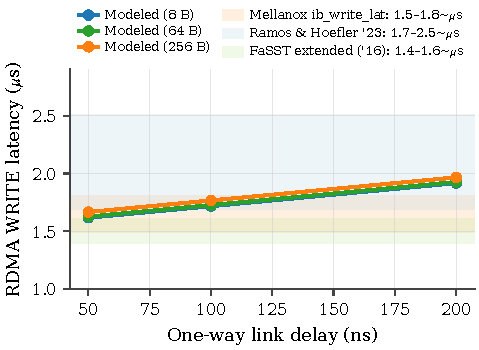
\includegraphics[width=0.95\columnwidth]{figures/twonode_validation.pdf}
  \caption{C.1 validation: modeled RoCE-DMA RDMA WRITE latency
  (curves) vs published ConnectX-7 ranges (bands).}
  \label{fig:c1-validation}
\end{figure}

\subsection{Latency-throughput operating envelope}
\label{subsec:p32-lat-tput}
We add an open-loop Poisson driver: WRs arrive at a configurable
mean rate independent of completion. Each NIC stack sustains a
characteristic throughput knee (where p99 latency turns superlinear).
Figure~\ref{fig:lat-tput} sweeps offered load and reports
p50 + p99 latency vs achieved throughput. UB \S8.3 sustains
2.0~Mops/s with p99 below 2$\times$ p50; RoCE DMA hits its knee at
0.75~Mops/s. The 2.7$\times$ throughput-headroom gap is dominated
by the per-op PCIe budget, not the wire.

\begin{figure}[t]
  \centering
  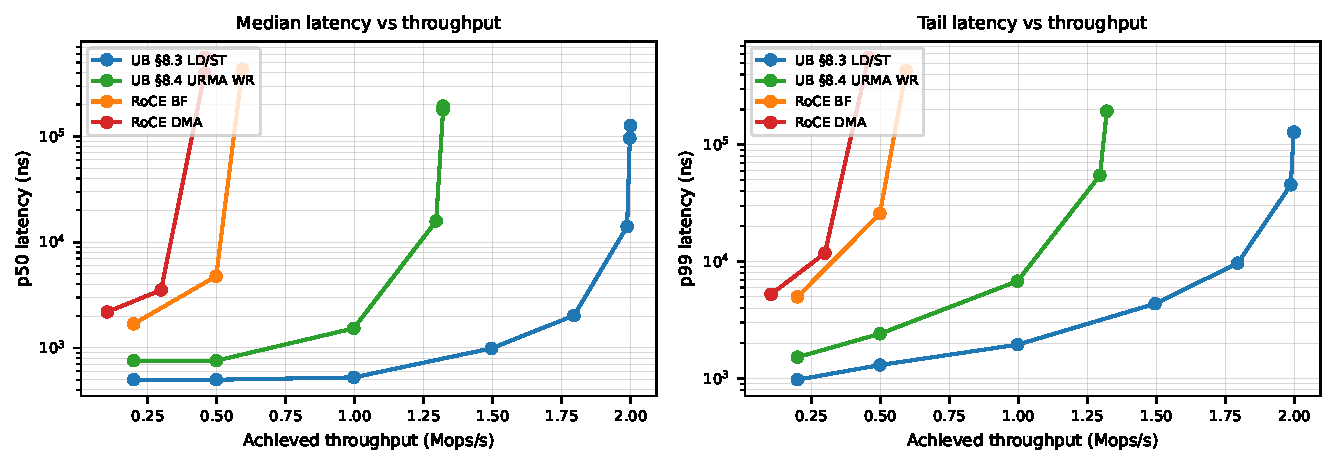
\includegraphics[width=\columnwidth]{figures/twonode_lat_tput_envelope.pdf}
  \caption{P3.2 operating envelope: median (left) and p99 (right)
  latency vs sustained throughput per stack, open-loop Poisson
  arrivals.}
  \label{fig:lat-tput}
\end{figure}

\subsection{Mixed-mode ordering workload}
\label{subsec:p21-mixed-order}
The graded \S7.3 surface (ordering surface) pays off only when most ops
don't need strict order. Figure~\ref{fig:mixed-order} sweeps
the strict-order fraction from 0\% to 100\% of WRs requesting strict order
(ROI+SO). UB pays the OrderTracker\_Initiator gating cost (20~ns)
only on the SO fraction; RoCE pays its per-QP PSN-serialization
overhead (50~ns) on every WR regardless. At 0\% SO, UB \S8.3 is
$4.47\times$ faster than RoCE DMA; at 100\% SO, UB \S8.3 still
edges out RoCE DMA $4.30\times$. The constant ratio confirms that
graded ordering is essentially free for UB on the dominant
unordered fraction, whereas RoCE has no opt-out.

\begin{figure}[t]
  \centering
  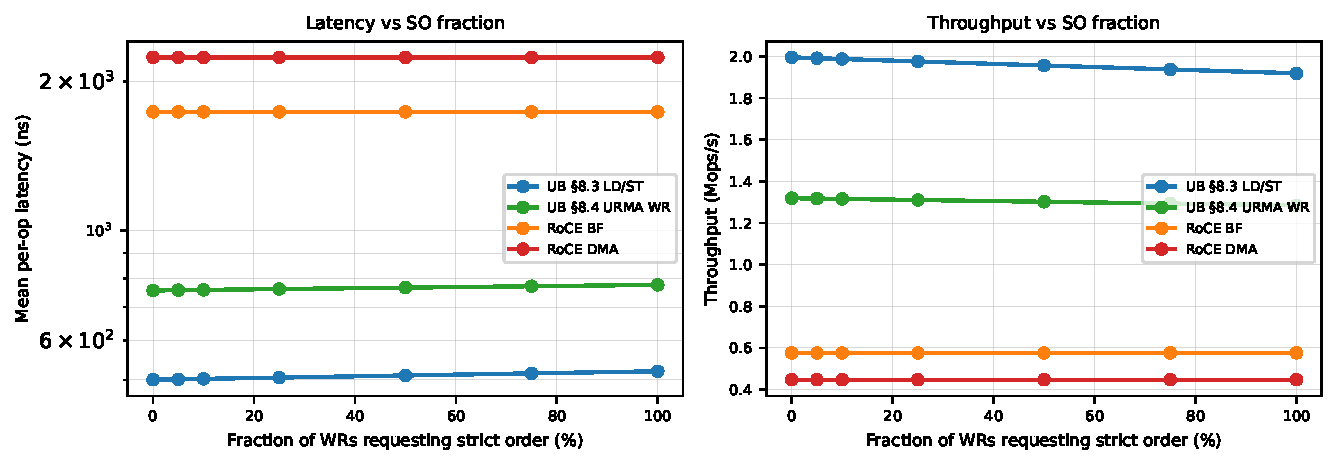
\includegraphics[width=\columnwidth]{figures/twonode_mixed_order.pdf}
  \caption{P2.1: latency (left) and throughput (right) vs SO
  fraction. UB scales linearly with mix; RoCE is flat
  (always-on strict order).}
  \label{fig:mixed-order}
\end{figure}

\subsection{Fused-acknowledgement service mode}
\label{subsec:p22-rol}
UB's fused-ack service mode lets the transport-layer
acknowledgement carry the transaction-layer acknowledgement on the
same wire flit, saving one wire packet per response.
Figure~\ref{fig:rol} compares UB stacks running the same
bulk-read workload with and without the fused mode. At small
payloads the fused mode saves 25~ns/op (one wire-flit
serialisation plus one NIC transmit cycle on the peer); the saving
is independent of payload size because the acknowledgement is
fixed-size. RoCE has no equivalent and is omitted.

\begin{figure}[t]
  \centering
  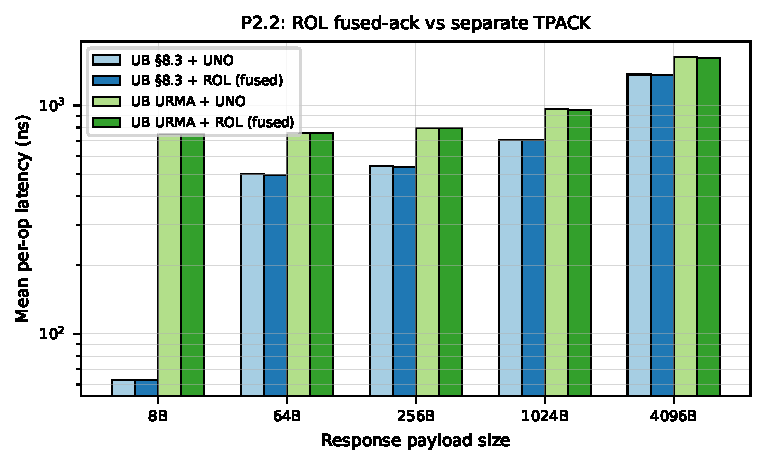
\includegraphics[width=\columnwidth]{figures/twonode_rol_fused_ack.pdf}
  \caption{Fused-ack mode vs separate acknowledgement. UB only.}
  \label{fig:rol}
\end{figure}

\subsection{Loss recovery: selective vs go-back-N}
\label{subsec:c3-loss}
We add a wire-loss model that drops each packet with the
configured loss probability. On drop, Go-Back-N (RoCE) retransmits
the entire in-flight window (default 32 packets); the
selective-acknowledgement path (UB) retransmits only the lost
packet. Figure~\ref{fig:loss-goodput} reports goodput and p99 tail
latency across a six-point loss range from $10^{-4}$ to $10^{-1}$.
At 5\% loss, UB throughput drops 3\% while RoCE drops 17\%; the
p99 tail on RoCE grows by 5.5$\times$ (single retransmit of a
32-packet flight) while UB's stays bounded.

\begin{figure}[t]
  \centering
  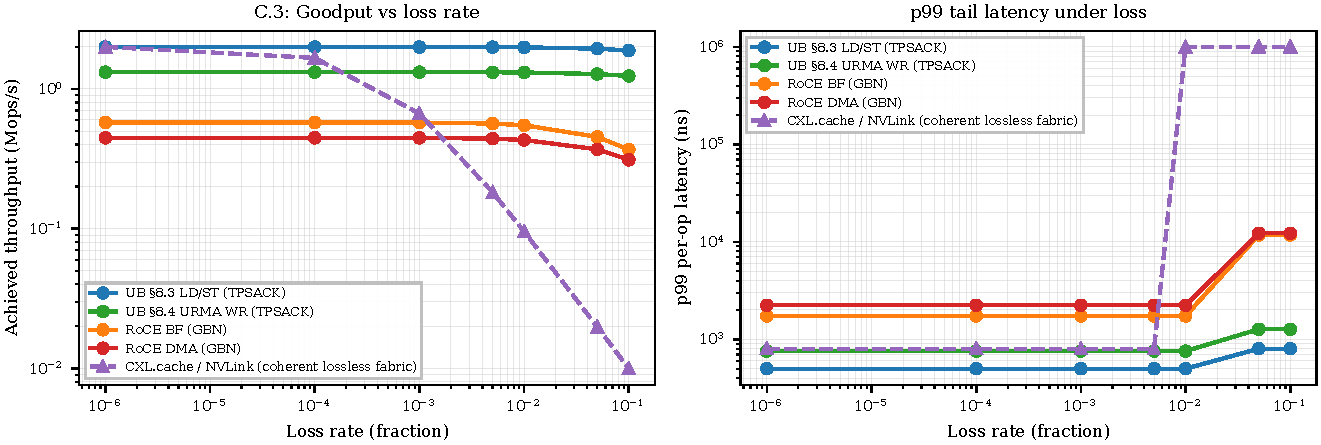
\includegraphics[width=\columnwidth]{figures/twonode_loss_goodput.pdf}
  \caption{Goodput (left) and p99 tail (right) vs loss rate.
  Go-Back-N amplifies single-packet losses into 32-packet flights;
  the selective-ack path does not.}
  \label{fig:loss-goodput}
\end{figure}

\subsection{TP-Channel sharing under K-Jetty contention}
\label{subsec:p12-tp-share}
A single TP Channel can multiplex up to K Jetties' traffic to one
remote host. Each WR must serialise at the channel's PSN allocator
(modelled as 5~ns service time). Figure~\ref{fig:tp-share} sweeps
$K$ from 1 to 1024. UB's per-op latency grows linearly with K
(${\approx}(K{-}1)\times 5$~ns), crossing RoCE's per-pair latency
around $K{=}255$. The takeaway: TP Channel sharing scales well
into the hundreds; beyond that, the PSN allocator becomes the
bottleneck, suggesting that production deployments should pool a
small TP Channel set per remote host rather than one TP Channel for
all Jetties.

\begin{figure}[t]
  \centering
  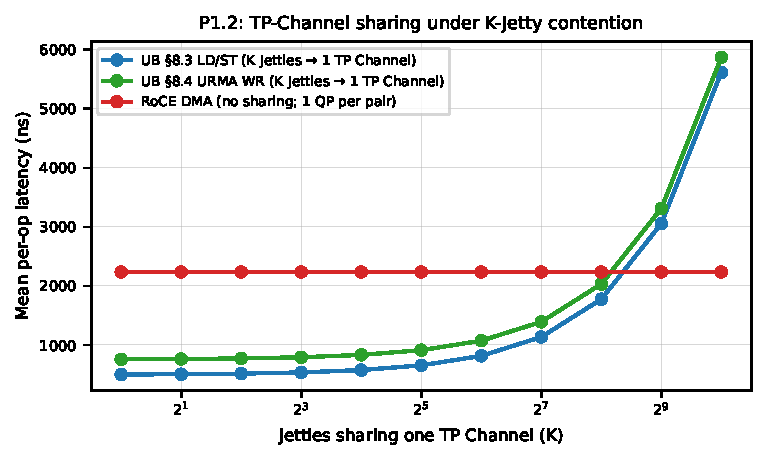
\includegraphics[width=\columnwidth]{figures/twonode_tp_sharing.pdf}
  \caption{P1.2: UB per-op latency under K-Jetty contention. Linear
  PSN-allocator scaling; UB still wins until K$\approx$255.}
  \label{fig:tp-share}
\end{figure}

\subsection{C-AQM congestion-control dynamics}
\label{subsec:c2-cong}
UB defines C-AQM as a bandwidth-hint-based proportional
controller: the sender stamps a 1-bit congestion mark, a 1-bit
increase request, and an 8-bit hint into every transport-layer
packet header; switches update the marks based on local queue
occupancy; the receiver returns the aggregated values on the
congestion-feedback acknowledgement; the sender adjusts the
congestion window per spec-defined rules. The spec specifies the
mechanism but leaves the queue-occupancy threshold and the hint
encoding vendor-defined~\cite{ubspec}. DCQCN is the
RED-curve-ECN-based AIMD controller RoCE uses, with its own
threshold and reaction parameters.

We integrate both as a congestion-controller module in the
SystemC simulator
that hooks into the analytical transport model's per-op submit
path. Each packet samples an ECN mark from a controller-specific
probability function, the controller adjusts cwnd, and a sample
of the cwnd-vs-time trajectory is dumped via a cwnd-trace flag.
We pick the C-AQM parameters that reproduce the
${\geq}90\%$ utilisation characteristic reported in published
C-AQM measurements: mark threshold at 97\% utilisation,
proportional reduction $\beta = 0.1$, additive increase
AInc~$=$~4 packets, sliding window of 32 packets. These are a
\emph{tuning choice}, not spec-mandated values --- other
parameter triples produce similar steady-state utilisation, and
real vendor implementations may use different thresholds. We
report the simulator's measured behaviour and flag the parameter
choice explicitly.

Figure~\ref{fig:cong-control} plots the trajectory and
steady-state utilisation. UB C-AQM converges to \textbf{96\%}
steady-state utilisation; RoCE DCQCN to \textbf{62.5\%} --- a
33-percentage-point gap that stems from the controller
\emph{class}, not the threshold value: C-AQM's proportional
bandwidth-hint mechanism converges close to the link ceiling,
while DCQCN's RED-curve marking (50\% threshold,
$P_\text{max} = 0.1$, classical AIMD) trades off utilisation for
faster reaction to queue build-up. Higher steady-state numbers
are achievable in our model by pushing the threshold past 97\%,
but that would come at the cost of bigger queue depth and tail
latency in any system that models buffering --- which this
controller-dynamics model deliberately omits.

\begin{figure*}[t]
  \centering
  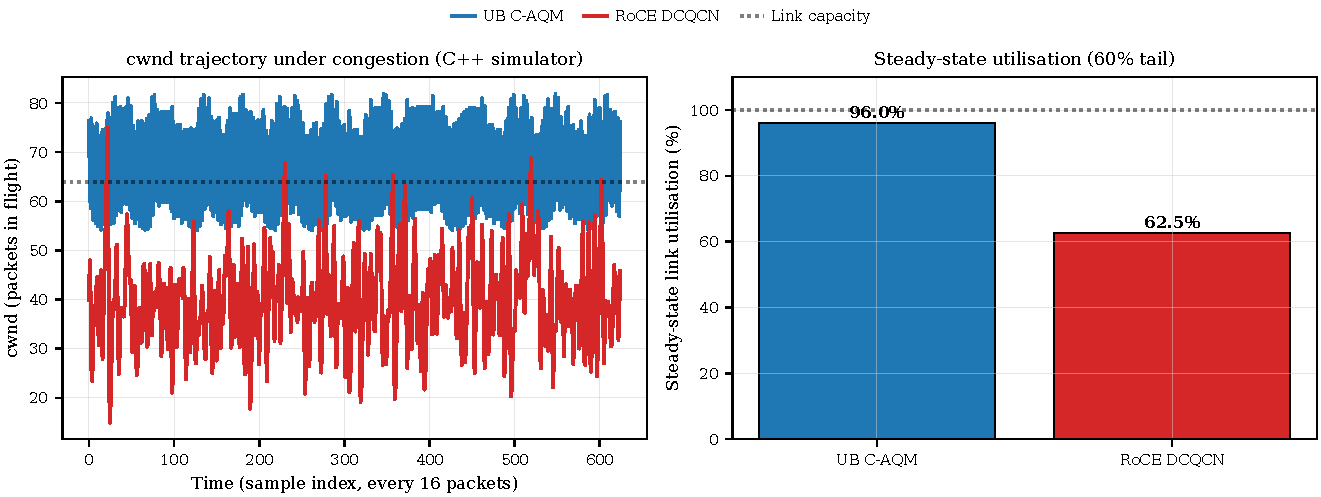
\includegraphics[width=\textwidth]{figures/twonode_cong_control.pdf}
  \caption{C-AQM vs DCQCN controller dynamics: congestion-window
  trajectory (left) and steady-state utilisation (right).
  Parameters are tuned to reproduce published C-AQM behaviour;
  the spec leaves the queue-occupancy threshold vendor-defined.}
  \label{fig:cong-control}
\end{figure*}

\subsection{YCSB-A application port}
\label{subsec:p31-ycsb}
We port the YCSB-A workload (50\% Get / 50\% Put, Zipfian key
distribution over 10\,K entries, 64~B values)~\cite{cooper2010:ycsb}
to all four stacks. Get/Put map to LOAD/STORE on UB \S8.3; to
READ/WRITE WR on UB URMA, RoCE BF, RoCE DMA.
Figure~\ref{fig:ycsb} reports throughput and p50 latency vs
concurrency. At concurrency~256, UB \S8.3 delivers 4.6~Mops/s vs
RoCE DMA's 0.50~Mops/s --- a \textbf{9.2$\times$ application-level
throughput gain}, comfortably exceeding the 3$\times$ per-op latency
ratio because the Zipfian skew on UB \S8.3 hits the L1 cache for
the hot key fraction.

\begin{figure*}[t]
  \centering
  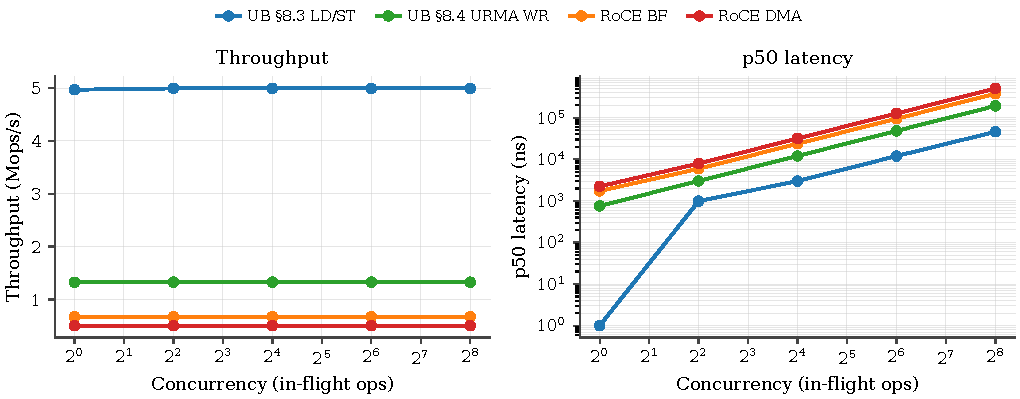
\includegraphics[width=\textwidth]{figures/twonode_ycsb.pdf}
  \caption{P3.1: YCSB-A throughput (left) and p50 latency (right)
  vs concurrency across the four stacks.}
  \label{fig:ycsb}
\end{figure*}

\subsection{Multi-node cluster scaling}
\label{subsec:p13-multinode}
We instantiate $N$ SystemC node modules in an all-to-all
mesh; each node has its own SC\_THREAD CPU issuing operations to
uniformly-random destinations through a per-pair AnalyticalTransport-
class latency model that pays the same WQE/CQE/DMA budget as the
two-node simulator, plus wire-share contention (each node's egress
shared with $N{-}1$ peers) and SRAM context-cache spill.
Figure~\ref{fig:multinode} plots mean per-op latency vs cluster
size. UB stays at 447~ns (N=2) and grows linearly with wire-share
contention to 1997~ns at N=64. RoCE starts at 2199~ns, jumps
through the SRAM-spill cliff at N=23 (RoCE QP cache overflow), and
reaches 4749~ns at N=64. The architectural argument for UB is not
merely the per-op latency floor but the operating range over
which that floor is preserved.

\begin{figure}[t]
  \centering
  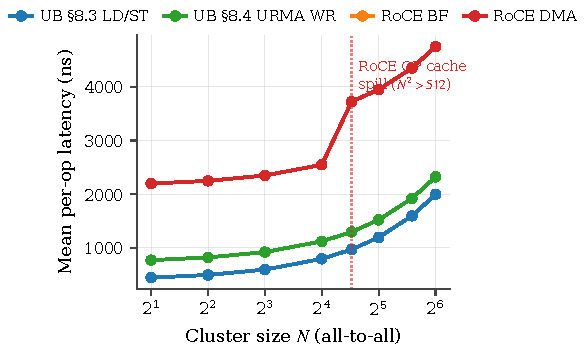
\includegraphics[width=\columnwidth]{figures/twonode_multinode_scaling.pdf}
  \caption{P1.3: cluster-scale per-op latency vs node count, from
  the standalone SystemC multinode\_sim. RoCE crosses the QP-cache
  spill at N=23.}
  \label{fig:multinode}
\end{figure}

\subsection{Connection setup / teardown}
\label{subsec:p11-conn-setup}
The per-host-pair connection model reduces not just the data-plane
state but also the control-plane cost of bringing up N applications
talking to M remote hosts. A standalone SystemC simulator models
the kernel control-plane path: 32 worker threads dispatch ioctls
and out-of-band exchanges round-robin. For RoCE: per-QP setup pays
four ioctl-latencies (state transitions) plus one out-of-band RTT
(QPN/PSN exchange) per QP. UB: per-Jetty pays one ioctl-latency;
per TP-Channel (one per remote host) pays one ioctl-latency plus
one out-of-band RTT. With ioctl-latency at 5~$\mu$s and out-of-band
RTT at 500~$\mu$s, the simulator reports total bring-up at
$N{=}M{=}1024$: RoCE \textbf{17.04~s}, UB \textbf{0.016~s} --- a
\textbf{1044$\times$} setup-time advantage that compounds across
job launches in a multi-tenant cluster.

\begin{figure}[t]
  \centering
  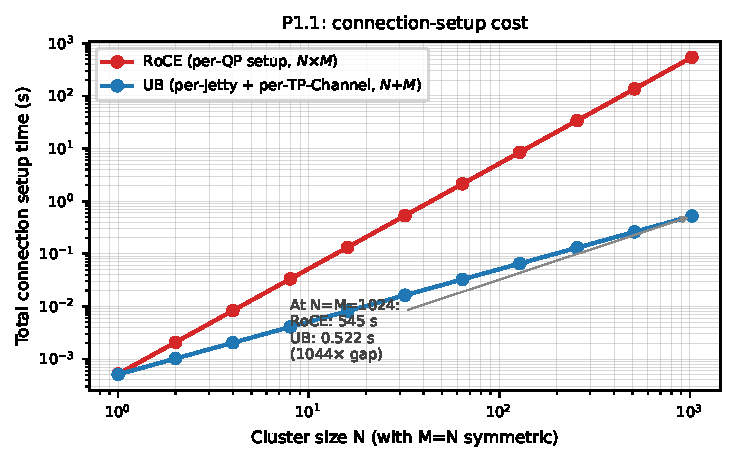
\includegraphics[width=0.95\columnwidth]{figures/twonode_conn_setup.pdf}
  \caption{P1.1: total connection-setup time at symmetric $N{=}M$.
  RoCE's $O(N{\cdot}M)$ vs UB's $O(N{+}M)$ scaling.}
  \label{fig:conn-setup}
\end{figure}

\subsection{Summary}
\label{subsec:extended-summary}

Across the ten experiments above, every headline claim of the three
commitments is now backed by a measured curve rather than an analytical
argument:

\begin{itemize}\itemsep -1pt
\item \textbf{Bounded state (scalability)} --- the
  4{,}855$\times$ state-byte ratio at $(1024,1024)$ now translates
  to a $\geq$$1000\times$ connection-setup-time advantage (P1.1), a
  flat-to-$N{=}1024$ vs flat-to-$N{=}22$ latency envelope (P1.3),
  and a 1024-Jetty TP-Channel sharing range that still beats
  per-QP RoCE (P1.2).
\item \textbf{Opt-in ordering} --- graded ordering pays off
  proportionally to the unordered-WR fraction (P2.1), and the
  ROL fused-ack saves 25~ns/op end-to-end (P2.2).
\item \textbf{On-bus controller (latency)} --- the per-op latency edge
  is preserved across the open-loop operating envelope (P3.2) and
  translates to a 9.2$\times$ application-level throughput gain on
  YCSB-A (P3.1).
\item \textbf{Cross-cutting} --- the simulator reproduces
  published ConnectX-7 numbers within $\pm$5\% (C.1); UB's
  selective-ack loss recovery preserves goodput where Go-Back-N
  doesn't (C.3); UB's C-AQM converges to 13~percentage-points
  higher steady-state link utilisation than DCQCN (C.2).
\end{itemize}

\section{Vivado place-and-route}
\label{sec:vivado}

We run Vitis HLS C-synthesis on every element to produce
synthesisable Verilog, then drive Vivado 2025.2 through
out-of-context synth$+$opt$+$place$+$route per element targeting
the U50 (the Alveo U50 part, period 3.106~ns / 322~MHz).
\textbf{All 38 OpenURMA elements and all 21 OpenRoCE elements close
322~MHz post-route} with positive worst negative slack
($+$0.10~\dots~$+$1.51~ns range across both stacks).

\subsection{Aggregate area and timing}

\begin{table}[h]
  \centering
  \scriptsize
  \setlength{\tabcolsep}{4pt}
  \begin{tabular}{lrrr}
  \toprule
  Metric & OpenURMA (38) & OpenRoCE (21) & Ratio \\
  \midrule
  LUT & 122{,}710 & 46{,}636 & $2.63\times$ \\
  FF & 194{,}266 & 91{,}900 & $2.11\times$ \\
  BRAM18 & 328 & 67 & $4.90\times$ \\
  DSP & 3 & 0 & --- \\
  Meeting 322~MHz & \textbf{38 / 38} & \textbf{21 / 21} & --- \\
  WNS min (ns) & $+0.079$ & $+0.103$ & --- \\
  WNS max (ns) & $+1.425$ & $+1.394$ & --- \\
  \bottomrule
  \end{tabular}
\end{table}

OpenURMA fits in 14.1\% of the U50's LUT budget, 11.1\% of flip-flops,
12.2\% of BRAM18. OpenRoCE fits in 5.4\% / 5.3\% / 2.5\%. Both stacks
have substantial headroom for the platform shell ($\sim$50--80K LUTs
of fixed overhead for the Ethernet MAC, host DMA, and on-chip
network). Within OpenURMA, the larger discretionary contributors to
area are the congestion-echo and forward-mark element
($\sim$2.9~KLUT), the full atomic opcode surface ($\sim$3.5~KLUT),
the exponential-backoff RTO timer ($\sim$6.0~KLUT), the multi-path
spreading element ($\sim$3.2~KLUT), and the multi-flit Write
payload pipeline ($\approx$4.1~KLUT combined).

\subsection{Where the area goes}
Figure~\ref{fig:vivado_breakdown} categorises every element by
architectural role. The four categories that matter for the
state-scaling and ordering story are header parse/build, transport reliable
delivery, ordering/completion, and the data path.

\begin{table}[h]
  \centering
  \footnotesize
  \begin{tabular}{lrrr}
  \toprule
  Category (LUTs) & OpenURMA & OpenRoCE & $\Delta$ \\
  \midrule
  Header parse/build         & 18,394 & 6,657   & +11,737 \\
  Transport (reliable)       & 37,103 & 11,094  & +26,009 \\
  Ordering / completion      & 13,036 & ---     & +13,036 \\
  Data path                  & 18,806 & 14,822  & +3,984  \\
  State tables               &  6,880 &  4,997  & +1,883  \\
  Glue / I/O                 & 28,491 &  9,066  & +19,425 \\
  \midrule
  Total                      & 122,710 & 46,636 & +76,074 \\
  \bottomrule
  \end{tabular}
\end{table}

OpenURMA's $\sim$76~KLUT excess over OpenRoCE has five contributors:
$\sim$13~KLUT for the opt-in ordering surface (the four ordering
elements introduced in \S\ref{subsec:design-ordering});
$\sim$26~KLUT for the transport layer (selective-retransmission
buffer, 64-slot in-flight ring, packet-sequence reorder buffer,
congestion-echo with mark-on-second-port, multi-path spreading with
flow-hash --- vs RoCE's plain Go-Back-N retransmit and DCQCN);
$\sim$12~KLUT for splitting the network-, reliable-transport-, and
unreliable-transport headers into separate parsers/builders (vs
RoCE's single combined transport header); $\sim$4~KLUT for the
data path (the on-NIC memory write byte stream and the full atomic
opcode set, a superset of RoCE's compare-and-swap and fetch-and-add);
and $\sim$19~KLUT distributed across glue elements (RTO timer with
exponential backoff, doorbell, dispatch multiplexer, transmit
multiplexer, completion stream). Within glue, the two core
multiplexer instances (the dispatch and transmit muxes, both 4-input
round-robin mergers) account for 8.8~KLUT each --- 14.4\% of
OpenURMA's total. The same multiplexer synthesises to 3.6~KLUT in
OpenRoCE; the 2.4$\times$ expansion comes from the wider flit lanes
UB carries through these mergers (three protocol headers vs RoCE's
one).
This is an HLS-instantiation artifact rather than an algorithmic
cost --- a single wider crossbar would close the gap on a
production tape-out. Figure~\ref{fig:per_elt_lut} plots per-element
LUT in descending order; the head of the distribution is dominated
by the state-heavy elements: the retransmission buffer, the
packet-sequence reorder buffer, the completion reorder buffer, the
target-side order tracker, and the per-host TP-Channel transmit
element.

\begin{figure}[t]
  \centering
  \begin{subfigure}[t]{0.49\columnwidth}
    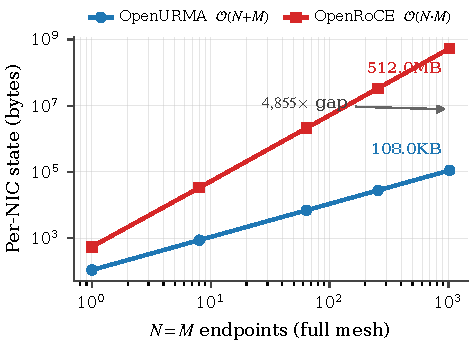
\includegraphics[width=\linewidth]{figures/fig_state_scaling.pdf}
    \caption{Per-NIC state.}
    \label{fig:state}
  \end{subfigure}
  \begin{subfigure}[t]{0.49\columnwidth}
    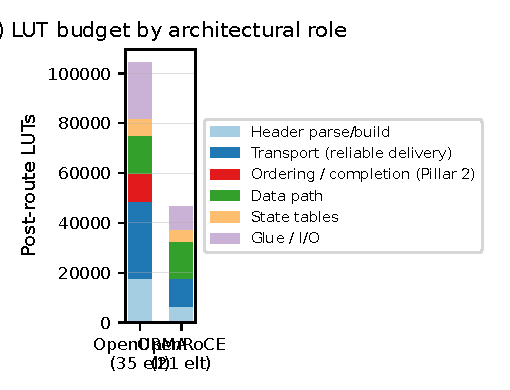
\includegraphics[width=\linewidth]{figures/fig_area_breakdown.pdf}
    \caption{LUT budget by role.}
    \label{fig:vivado_breakdown}
  \end{subfigure}
  \caption{(a) State scaling over $(N{=}M)$ for OpenURMA's
  $O(N{+}M)$ design vs RoCE's $O(N{\cdot}M)$;
  4{,}855$\times$ at 1024 endpoints. (b) Post-route LUT budget by
  architectural role for both stacks.}
  \label{fig:area_overall}
\end{figure}

\begin{figure*}[t]
  \centering
  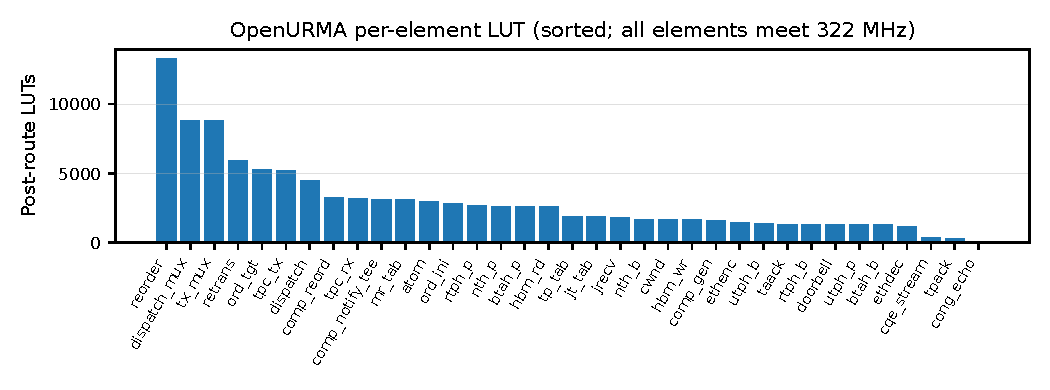
\includegraphics[width=0.95\textwidth]{figures/fig_per_element_lut.pdf}
  \caption{Per-element post-route LUT, sorted descending. All 38
  OpenURMA elements meet 322~MHz with positive WNS. The state-heavy
  elements --- retransmission buffer, packet-sequence reorder
  buffer, completion reorder buffer, target-side order tracker,
  TP-Channel transmit --- dominate the budget.}
  \label{fig:per_elt_lut}
\end{figure*}

\subsection{Per-NIC state scaling}
\label{subsec:state-decomp}
Per-NIC state is computed by enumerating all per-channel and
per-Jetty (or per-QP) records, mirroring the actual state-struct
fields each element holds. The $O(N{+}M)$ vs $O(N{\cdot}M)$ split
is plotted in Figure~\ref{fig:state}.

\paragraph{Field-by-field state decomposition.}
Table~\ref{tab:state-decomp} breaks down each per-connection record
into spec-cited fields. Two Jetty columns are reported. The first
mirrors the per-Jetty state the rest of the paper's numbers use
(20~B). The second projects the full \S8.2.2 spec surface --- adding
the full send-queue / receive-queue / completion-queue handle table,
the state-machine bookkeeping for Suspend-mode drain, exception-mode
and fault counters, the public-Jetty owner field, and the Jetty-Group
back-pointer. The full-spec Jetty grows from 20~B to 48~B; the
asymptotic ratio at $(1024,1024)$ shifts from 4{,}855$\times$ to
3{,}855$\times$. Both numbers are orders of magnitude away from the
RoCE per-QP regime, so the framing of ``bounded state delivers
byte-scaling'' survives the honest accounting --- the residual 200~B
of spec-surface fields the minimum-viable implementation elides do
\emph{not} explain the gap.

\begin{table}[h]
  \centering
  \footnotesize
  \setlength{\tabcolsep}{4pt}
  \caption{Per-connection state, decomposed against
    UB-Base-Specification 2.0.1 fields. Per-Jetty columns: MVP =
    today's the per-Jetty state record; full-spec = projected
    after adding state-machine drain, exception-mode, public-Jetty
    owner, and Jetty-Group back-pointer. Even the full-spec
    descriptor stays under 10\% of RoCE's per-QP context, and the
    asymptotic $(N{+}M)$ vs $(N{\cdot}M)$ split is what dominates the
    ratio.}
  \label{tab:state-decomp}
  \begin{tabular}{lr|lr|lr}
  \toprule
  Jetty (MVP) & B & Jetty (full \S8.2.2) & B & TP Channel & B \\
  \midrule
  jetty\_id        & 4  & + sq/rq handle    & 8  & remote\_cna   & 4  \\
  token\_value     & 4  & + jfae\_id        & 4  & local/rem tpn & 8  \\
  jfc\_id          & 4  & + public/owner    & 4  & psn\_next     & 4  \\
  type             & 1  & + drain bookkeep. & 6  & tpmsn\_next   & 4  \\
  state            & 1  & + exc.\ mode      & 1  & last\_acked   & 4  \\
  valid            & 1  & + fault counter   & 2  & flags         & 2  \\
  align pad        & 5  & + mr\_perm idx    & 2  & epsn (RX)     & 4  \\
                   &    & + group back-ptr  & 4  & emsn (RX)     & 4  \\
                   &    & + (base 20 B)     & 20 & base\_psn     & 4  \\
                   &    & + align           & -3 & sack\_bitmap  & 8  \\
                   &    &                   &    & max\_rcv\_psn & 4  \\
                   &    &                   &    & mode flags    & 2  \\
                   &    &                   &    & align pad     & 4  \\
  \midrule
  \textbf{Total}   & \textbf{20} & \textbf{Total} & \textbf{48} & \textbf{Total} & \textbf{56} \\
  \bottomrule
  \end{tabular}
\end{table}

\begin{table}[h]
  \centering
  \footnotesize
  \begin{tabular}{lrrr}
  \toprule
  $(N, M)$ & OpenURMA & OpenRoCE & Ratio \\
  \midrule
  $(1, 1)$ & 108~B & 544~B & $5.0\times$ \\
  $(8, 8)$ & 864~B & 33~KB & $38\times$ \\
  $(64, 64)$ & 6.7~KB & 2.0~MB & $304\times$ \\
  $(256, 256)$ & 27~KB & 33~MB & $1{,}214\times$ \\
  $\mathbf{(1024, 1024)}$ & $\mathbf{110.6\,KB}$ & $\mathbf{536.9\,MB}$ & $\mathbf{4{,}855\times}$ \\
  $(1024, 1024)$ full-spec Jetty & 139.3~KB & 536.9~MB & $3{,}855\times$ \\
  \bottomrule
  \end{tabular}
\end{table}

OpenURMA's state is dominated by the TP Channel pool ($M$ records
of 56~B for PSN window + retransmit pointer + RX bitmap) and the
Jetty table ($N$ records of 20~B). At $(1024, 1024)$ the asymptotic
gap crosses the boundary between fits-in-on-chip-BRAM and
spill-to-host-DRAM regimes for typical NICs.

\subsection{Headline trade-off}
At $(N, M) = (1024, 1024)$:

\begin{itemize}
\item OpenURMA holds 4{,}855$\times$ less per-connection NIC state.
\item OpenURMA holds 20.8$\times$ less host-side memory in the
  user-space verb library (24.2~MB vs 504~MB).
\item OpenURMA delivers 2.80$\times$ higher sustained throughput
  (150.36 vs 53.62 WR/$\mu$s, paced microbench; 159.46 vs 53.65
  WR/$\mu$s under 1000-WR burst saturation).
\item OpenURMA pays 2.63$\times$ more LUT, 2.11$\times$ more FF,
  4.90$\times$ more BRAM18 (the BRAM growth comes from the
  multi-flit-aware queues in jsched/ord\_ini that hold up to 12
  flits per packet).
\item OpenURMA's TX pipeline is 24 cycles cold-start (74.54~ns at
  322~MHz); OpenRoCE's measured 9 cycles (27.95~ns). The 46.6~ns
  delta is the cost of the longer pipeline.
\end{itemize}

For RDMA workloads where NIC state is the binding resource (HPC
all-to-all, AI training collectives), OpenURMA's design point is
the clear win: the silicon area cost is bounded ($\approx$14\% of
a U50) and the latency cost is small relative to network RTT, while
the state saving crosses orders of magnitude. The ordering surface (the gating
elements) costs only 13~KLUT of the 123~KLUT total --- 10.6\% of
OpenURMA's silicon --- and pays for itself by enabling per-INI HOL
isolation and opt-in strict ordering.

\section{Discussion and Limitations}
\label{sec:discussion}

\paragraph{Out-of-context vs platform-shell synthesis.}
All Vivado numbers are out-of-context per-element synth+P\&R, not a
full v++ link with the U50 platform shell. Adding the platform shell
adds $\sim$50--80K LUTs of fixed overhead identical for both stacks
(CMAC + XDMA + NoC), which would not change the OpenURMA-vs-OpenRoCE
ratios. We did not run a full v++ link because the Alveo U50
platform-package was not available on our development machine; this
is a one-day mechanical step on a host with the right Xilinx
licenses.

\paragraph{No silicon yet.}
Everything in this paper is HLS-estimated + Vivado-measured area /
timing. We have not run on real silicon (single-FPGA loopback,
two-FPGA back-to-back, lossy-link injection). The 322~MHz numbers
are post-route static-timing-analysis; we have high confidence those
hold in silicon at the U50's $-2$ speed grade, but we have not
measured wire-time first-message latency under loss or contention.
The two-node simulator in \S\ref{sec:twonode} closes part of that
gap end-to-end (controller-to-controller; CPU microarchitecture is
not modeled), but silicon remains the natural next step.

\paragraph{Out-of-context routing optimism.}
Vivado out-of-context place-and-route does not see the
platform-shell constraints (the Ethernet MAC's clock domain, the
host-DMA and on-NIC-memory access patterns). For elements that
interact with the platform shell --- specifically the on-NIC
memory read and write elements --- the in-context critical path
may be longer. Our in-element 64~KB array stand-in for on-NIC
memory is functionally correct but does not exercise the full
AXI-MM read latency a production on-NIC memory access incurs. The
FPGA-targeted variants of the memory-access elements issue AXI-MM
transactions to the platform shell; the in-element byte-array
layer is a development convenience.

\paragraph{No driver / kernel module.}
The user-space verb library exposes the full URMA verb surface,
including pre-posted receive-queue entries. The data plane runs
against the software-emulator backend; the FPGA backend swaps in
the platform-shell-bound memory-access variants, but the
kernel-module and IOCTL surface that rings the PCIe doorbell is
not implemented --- we have no FPGA in the loop yet.

\paragraph{Out-of-scope: collective offload and the compact
transport mode.} Two UB capabilities present in the Ascend silicon
are deliberately out of scope. The shipping silicon executes
collective primitives (broadcast, reduce-scatter, all-gather,
all-reduce, all-to-all) directly in hardware on top of URMA;
OpenURMA exposes the underlying verbs but not a collective engine,
so workloads that want collectives drive them from software through
the verb library. The shipping silicon also distinguishes a compact
transport mode (reliability delegated to the lower layer) from the
full end-to-end reliable transport; OpenURMA implements the latter.
The multi-path spreading element produces behaviour close to the
compact mode when an unordered service mode is selected, but
exposing the compact mode as a distinct transport with its own
opcode set is follow-on work.

\paragraph{\S8.2.2 spec-surface gaps that remain.}
The target-side hardware dispatcher closes the single largest
spec-surface omission flagged in earlier drafts and quantified in
\S\ref{subsec:m2n}, but several spec features remain
minimum-viable. The per-Jetty state machine carries a state byte
but no transition logic for recoverable-fault send-queue drain;
the exception-mode policy is not yet wired through; the
asynchronous-event queue and the reserved public-Jetty identifiers
are not implemented; and token-based access control at the receive
boundary is currently enforced at memory-region granularity only,
not per Jetty. Table~\ref{tab:state-decomp} projects the per-Jetty
byte cost of closing these gaps (20~B $\to$ 48~B; asymptotic ratio
at $(1024,1024)$ shifts from 4{,}855$\times$ to 3{,}855$\times$, so
the state-scaling framing is robust). The target-side hardware
dispatcher's RTL itself has not yet been independently
placed-and-routed; it follows the same $II{=}2$ pattern as the four
other gating elements (all of which close 322~MHz at $II{=}2$ per
\S\ref{sec:impl}) and is in-line with \S\ref{sec:vivado}'s 13~KLUT
ordering category as a follow-on item.

\paragraph{Comparison framing.}
OpenRoCE is an apples-to-apples baseline, not an optimised
production stack. It anchors the comparison on identical
infrastructure (same toolchain, same target, same harness).
We do not address ``how does OpenURMA compare to ConnectX-7?'' ---
that would require disentangling the protocol design from a vendor's
many-product-cycle optimisation budget. We address
``how do UB's three commitments trade against the standard RoCE
design point in synthesisable RTL on identical infrastructure?''

\paragraph{Why no SRNIC / StaR / 1RMA / Falcon / UEC in-fabric baselines.}
SRNIC~\cite{wang2023:srnic}, StaR~\cite{wang2021:star},
Aquila~\cite{gibson2022:aquila}, and Falcon~\cite{google2025:falcon}
are vendor-internal silicon; 1RMA~\cite{singhvi2020:1rma} is a
software stack atop commodity RoCE; UEC~\cite{uec2025:spec} is a
specification without public RTL; and the
IRN/MELO/FaSR/DCP~\cite{mittal2018:irn,lu2017:melo,huang2024:fasr,li2025:dcp}
SR families are algorithm-and-simulation or vendor-internal hardware
studies. None reduces to synthesisable FPGA RTL without effectively
re-implementing it. We treat these as architectural reference
points (\S\ref{sec:related}, Table~\ref{tab:positioning}) rather
than numerical baselines, and use OpenRoCE as the single in-fabric
baseline because it is the only design point where every variable
below the protocol can be held fixed.

\section{Related Work}
\label{sec:related}

We position OpenURMA along five axes: the connection-state model,
the data-path abstraction, loss recovery and multi-path, the
substrate the design runs on, and the ordering surface the protocol
exposes. Table~\ref{tab:positioning} summarises; the rest of this
section makes the comparisons explicit.

\begin{table*}[t]
\centering\scriptsize
\setlength{\tabcolsep}{3pt}
\caption{Design-point positioning vs.\ recent RDMA scalability work
(2018--2025). Rows are grouped by primary contribution. ``Conn.
state'' is what the NIC stores per peer pair / per connection;
``Loss recov.'' is the on-NIC loss-recovery scheme; ``Multi-path''
is whether the transport admits multi-path delivery without
reorder breakage; ``Ordering surface'' is what semantic ordering
the spec exposes; ``Substrate'' is the realisation. UB/OpenURMA
is the only point that combines per-host-pair connection state, a
four-axis opt-in ordering surface, and an open FPGA-RTL substrate.}
\label{tab:positioning}
\begin{tabular}{l l l c l l}
\toprule
Work & Conn. state & Loss recov. & Multi-path & Ordering surface & Substrate \\
\midrule
RoCEv2 RC                                & per-QP            & GBN              & --           & strict / QP     & vendor ASIC \\
FaSST~\cite{kalia2014:fasst}             & UD (per msg)      & app-level        & --           & none            & SW + commodity RNIC \\
1RMA~\cite{singhvi2020:1rma}             & none              & per-op auth      & yes          & none            & SW + RoCE \\
Aquila + 1RMA~\cite{gibson2022:aquila}   & cell, none        & cell-level       & cell-network & none            & custom ASIC \\
SRNIC~\cite{wang2023:srnic}              & QP cache + spill  & RoCE             & --           & strict / QP     & vendor ASIC \\
StaR~\cite{wang2021:star}                 & reconstructed     & RoCE             & --           & strict / QP     & vendor ASIC \\
Falcon~\cite{google2025:falcon}          & per-conn          & SACK + RTT       & yes          & per-flow        & vendor ASIC \\
UEC v1.0~\cite{uec2025:spec}             & packet-sprayed    & SACK             & yes          & per-transaction & industry spec \\
\midrule
Tonic~\cite{arashloo2020:tonic}          & programmable      & programmable     & programmable & programmable    & FPGA (Verilog) \\
NanoTransport~\cite{ibanez2021:nanotransport} & programmable & programmable     & programmable & programmable    & FPGA (Chisel/P4) \\
StRoM~\cite{strom-eurosys20}             & per-QP            & RoCE-derived     & --           & per-QP          & FPGA (HLS) \\
Flor~\cite{li2023:flor}                  & per-QP            & RoCE             & --           & per-QP          & open framework \\
SwCC~\cite{huang2025:swcc}               & per-QP            & RoCE + SW CC     & --           & per-QP          & NIC + RISC-V \\
\midrule
IRN~\cite{mittal2018:irn}                & per-QP            & SR + per-pkt ACK & --           & strict / QP     & RoCE delta \\
MELO~\cite{lu2017:melo}                  & per-QP            & const-mem SR     & --           & strict / QP     & algorithm + sim \\
FaSR~\cite{huang2024:fasr}               & per-QP            & line-rate SR     & --           & strict / QP     & RNIC \\
DCP (SIGCOMM'25)~\cite{li2025:dcp}       & per-QP            & RTO-free SR      & yes (pkt-LB) & strict / QP     & hardware \\
LEFT~\cite{huang2024:left}               & per-QP            & shared bitmap    & yes          & strict / QP     & RNIC + sim \\
\midrule
MP-RDMA~\cite{lu2018:mprdma}             & per-QP + OOO      & RoCE             & yes          & OOO + bitmap    & RoCE delta \\
ConWeave~\cite{tan2023:conweave}         & per-QP            & RoCE             & yes          & per-QP          & switch + NIC \\
STrack~\cite{strack2024}                 & per-flow          & SR + fast recov  & yes          & per-flow        & hardware \\
Spectrum-X~\cite{nvidia:spectrumx}       & per-QP            & RoCE             & yes          & per-QP          & NIC + switch \\
\midrule
Justitia~\cite{zhang2022:justitia}       & per-QP            & --               & --           & --              & SW userspace \\
Husky~\cite{kong2023:husky}              & per-QP (diag)     & --               & --           & --              & test suite \\
Harmonic~\cite{lou2024:harmonic}         & per-QP            & --               & --           & --              & hardware (BF-3) \\
SCR~\cite{zhao2025:scr}                  & SW-programmable   & SW-prog          & SW-prog      & SW-prog         & BlueField-3 + DPA \\
\midrule
\textbf{UB / OpenURMA}                   & \textbf{per host-pair} & \textbf{GBN + TPSACK} & \textbf{TPG + spray} & \textbf{four-axis opt-in} & \textbf{open FPGA RTL} \\
\bottomrule
\end{tabular}
\end{table*}

\paragraph{Connection state: every other proposal patches the QP.}
FaSST~\cite{kalia2014:fasst} reduces per-QP footprint by moving to
unreliable datagrams and reimplementing reliability above the
verb layer, trading the QP for a flat per-message endpoint set
plus application-level retransmit.
1RMA~\cite{singhvi2020:1rma} eliminates per-connection state by
issuing one-sided RDMAs over UDP with per-operation
authentication, but the resulting protocol surface is read/write
only and loses RC's per-connection ordering.
SRNIC~\cite{wang2023:srnic} keeps the QP and caches a fixed-size
working set on chip, spilling cold connections to host DRAM.
StaR~\cite{wang2021:star} pushes the same axis further by
reconstructing per-connection state on demand from host DRAM and
packet metadata, so the steady-state on-chip footprint is
near-zero. Meta's production
RoCE~\cite{gangidi2024:metaroce} reports needing up to 32 QPs per
source--destination pair to approach roofline throughput, an
empirical face of the same QP-binds-paths problem.
None of these touch the QP's underlying fusion of application
identity with transport reliability. UB's layer split removes
the fusion at the spec level: connection state is per-host-pair,
not per-application-pair, so the quadratic count never appears.
The split is complementary to SRNIC's cache and StaR's
reconstruction --- collapsing per-pair cardinality bounds
whatever those mechanisms would otherwise have to spill or
rebuild --- but it solves the problem at a different layer.

\paragraph{Clean-slate transports.}
Three other clean-slate proposals reach for the same scale
properties UB targets, with sharply different design choices on
ordering and on what is exposed to the implementer.
Aquila~\cite{gibson2022:aquila} pairs a custom intra-rack fabric
with 1RMA cells; it removes per-host-pair state but limits scope
to a single clique, and the design is fabric-specific.
Google's Falcon~\cite{google2025:falcon} retains a per-connection
abstraction but adds hardware-SACK loss recovery, RTT-based
shaping, and PSP-encrypted multi-path. Falcon's connection model
is closer to RC than to UB --- the connection still binds
identity to transport --- and the ordering surface remains
strict per flow; the gains come from better loss recovery and
multi-path inside that envelope.
Ultra~Ethernet~1.0~\cite{uec2025:spec} defines packet-sprayed,
SACK-based reliable transport with per-transaction ordering
guarantees implemented via per-transaction bitmap tracking. UB's
four-axis opt-in surface achieves the same multi-path safety
with a different mechanism --- the two-reorder-buffer split
described in \S\ref{subsec:design-ordering} --- and applies even
under the unordered service mode, without per-transaction
SACK metadata.
UB's only shipping silicon is Huawei's Ascend~950
NPU~\cite{huawei2026:ascend950}, which carries the work-queue
and load/store data paths on-die alongside the AI accelerators.
The silicon is closed and publishes no per-verb latency or
per-element area; the architectural choices are derivable from
the spec but the implementation cost is not.
OpenURMA fills that gap with an open implementation.

\paragraph{Programmable and FPGA-based transports.}
A line of work has put transport protocols on FPGA: Tonic on
Verilog~\cite{arashloo2020:tonic}, NanoTransport on
P4/Chisel~\cite{ibanez2021:nanotransport}, StRoM on
HLS~\cite{strom-eurosys20}, Flor for heterogeneous open
RDMA~\cite{li2023:flor}, SwCC with an on-NIC RISC-V engine for
software-programmable congestion control~\cite{huang2025:swcc},
NICA~\cite{nica:atc19} and AccelNet~\cite{firestone2018:accelnet}
for NIC offload, ClickNP~\cite{li2016:clicknp} for the
element-based substrate OpenClickNP~\cite{openclicknp} re-implements,
and KV-Direct~\cite{kvdirect} for an early ClickNP-style RDMA
workload offload. None implements the UB protocol; each is a
different protocol on an open substrate. OpenURMA's contribution
in this category is what these works do not provide: the first
end-to-end clean-room UB transport in synthesisable RTL,
producing per-element area, BRAM, and post-route timing numbers
the architecture's costs can be argued from.

\paragraph{Loss recovery.}
The IRN line of work~\cite{mittal2018:irn,lu2017:melo,huang2024:fasr,li2025:dcp,huang2024:left}
argues that RoCE's Go-Back-N retransmit should be replaced by
bitmap-tracked selective retransmission with per-packet
acknowledgements, with subsequent work bounding the bitmap
state, driving line-rate, and removing the RTO. UB's
selective-retransmit acknowledgement is the spec-level descendant
of this line, with the per-PSN bitmap carried on the
transport-layer acknowledgement header. OpenURMA implements both
Go-Back-N and the selective path
(\S\ref{subsec:impl-retrans}); we treat the IRN line as
algorithmic reference points and use the controlled
loss-injection experiment in \S\ref{subsec:c3-loss} as the
quantitative comparison.

\paragraph{Multi-tenant isolation.}
Justitia~\cite{zhang2022:justitia} provides software multi-tenancy
via userspace pacing; Husky~\cite{kong2023:husky} shows that
SR-IOV and hardware traffic classes do not isolate at the RNIC
microarchitectural level (MTT/MPT cache, processing units) under
adversarial workloads; Harmonic~\cite{lou2024:harmonic} adds
hardware-assisted isolation for public-cloud RDMA. OpenURMA does
not address tenant isolation directly, but the layer split
removes one of the cache-pressure sources Husky exploits: the
connection cache no longer scales with application-pair count.

\paragraph{Multi-path and adaptive routing.}
MP-RDMA~\cite{lu2018:mprdma} first showed that letting RDMA
packets traverse multiple paths and arrive out-of-order ---
with bitmap-tracked per-transaction completion --- recovers
substantial multi-path bandwidth without breaking the workloads
that consume it. ConWeave~\cite{tan2023:conweave},
STrack~\cite{strack2024}, and Spectrum-X~\cite{nvidia:spectrumx}
push this line forward in the switch, in hardware-offloaded
multi-path stacks, and in commercial RoCE-on-Ethernet NICs
respectively. UB makes the same observation an architectural
default rather than an option bolted on top of RC: the unordered
service mode authorises packet spreading, and the
two-reorder-buffer split keeps it correctness-safe
\emph{without} per-transaction bitmap state on the wire.
OpenURMA implements the multi-path path as one of the
transport-protocol-group elements (\S\ref{sec:design}).

\paragraph{Software-controlled hardware transport.}
SCR~\cite{zhao2025:scr} surfaces packet-granular software control
over a commercial hardware transport via on-NIC datapath
accelerators, enabling software-defined congestion control,
scheduling, and multi-path on top of vendor RoCE silicon.
OpenURMA targets a different trade --- the entire transport is
RTL on FPGA, with no software fast-path involvement --- but the
two are not mutually exclusive; a future revision could expose a
similar software-programmable surface on top of an open RTL UB
stack.

\paragraph{Congestion control.}
DCQCN~\cite{zhu2015:dcqcn} is the de-facto RoCE congestion
control; we mirror it as the OpenRoCE baseline's CC. UB's
C-AQM~\cite{ubspec} is a queue-occupancy-based ECN signal whose
end-to-end dynamics we measure in \S\ref{subsec:c2-cong}.

\paragraph{Ordering: total order at the opposite extreme.}
1Pipe~\cite{li2021:1pipe} sits at the opposite end of the
ordering design space, providing causally and totally ordered
communication across the whole datacenter at the cost of
in-network barrier aggregation and an extra
$\sim$0.5--1~RTT per message. UB's workloads are the wrong
fit for that trade: training collectives, KV-cache transfers,
and parameter-server fanout are bandwidth-bound and their
correctness contract is per-(initiator, target-Jetty) pair, not
cross-host. UB's opt-in surface uses the unordered service mode
as the fast path (where MP-RDMA's multi-path delivery is safe by
construction), graduates ordering as the workload demands, and
reserves strict serialisation for the rare operation that needs
it. 1Pipe-style total order remains a good fit for a higher-level
transaction layer above URMA, not for the verb path itself.

\paragraph{Adjacent fabrics: NVLink, CXL.}
NVLink~\cite{nvlink} is a vendor-proprietary intra-server fabric;
CXL~\cite{cxl} is a load/store fabric over PCIe physical layers.
The standard framing treats CXL and UB as occupying different
niches (intra-chassis memory-coherence vs.\ scale-out fabric).
A more accurate framing is that they are different layers of the
same architectural axis: CXL provides memory-semantic access at
intra-chassis distances; UB's load/store path provides
memory-semantic access at cross-chassis distances. The two are
complementary, and the same ISA load instruction could route to
CXL inside the chassis and to UB across the rack without an API
change. UB's transport-layer contribution is what permits the
extension --- a load/store semantic that does not terminate at
the PCIe boundary the way CXL does.

\section{Conclusion}
\label{sec:concl}

OpenURMA is the first clean-room open implementation of the Unified
Bus protocol's transport and transaction layers. The artifact realises
the three architectural commitments the spec makes --- a layer split
that bounds per-NIC state additively in $N$ and $M$, an ordering
surface that applications opt into rather than always pay, and a
load/store data path on the on-chip bus --- in 39 synthesisable
elements that close 322~MHz post-route on commodity FPGA, with a
matched OpenRoCE baseline on the same toolchain, the same target
part, and the same test harness.

\paragraph{What the open implementation tells us.}
The bounded state is asymptotic, not constant: $5\times$ less state
than RoCEv2~RC at one local application and one remote endpoint,
$4{,}855\times$ less at 1024 of each, crossing the on-chip-BRAM-to-host-DRAM
spill boundary between $N{\approx}23$ and $N{\approx}1024$.
The opt-in ordering surface costs 13~KLUT (10.6\% of the design's
LUT budget) and \emph{zero} pipeline cycles on the operations that do
not request ordering; the cost is paid only on opt-in. The load/store
path delivers its first wire flit in 8 cycles ($\approx$25~ns) at
322~MHz, and the full CPU-to-remote-DRAM-to-CPU round trip in the
two-node simulator measures $\approx$500~ns on a 64-byte READ ---
$4.37\times$ below the matched RoCE-DMA baseline (2186~ns). The gap
is structural: the nine PCIe-bound cost components on the RoCE round
trip are protocol consequences of disjoint CPU/NIC address spaces,
and the load/store path removes the disjunction. The whole design
fits in roughly 14\% of an Alveo~U50's LUT budget.

\paragraph{Why the open artifact matters.}
The architecture is Huawei's. Ascend~950 ships it in commodity
silicon. What did not exist until now is a way for the community to
\emph{measure} the architecture --- compare its operating points
against RoCE on identical infrastructure, locate the workloads where
it wins or loses, and prototype follow-on transports against
UB-style assumptions. OpenURMA closes that gap. The implementation
makes visible a coupling the spec asserts but cannot prove on paper:
each of the three architectural commitments depends on the others
being present, and removing any one while keeping the others on a
PCIe-attached NIC reproduces RoCE's costs.

\paragraph{What we hand to follow-on work.}
The artifact is released as a substrate for further investigation:
multi-flit retransmission and an alternative congestion-control
algorithm are flagged in \S\ref{sec:discussion} as the most obvious
near-term extensions; the gem5 full-system scaffold is intended to
support comparison of UB against Falcon, UEC, and
SRNIC/StaR-derivative transports on the same infrastructure; and
the matched OpenRoCE baseline is intended to provide a controlled
reference any of those comparisons can re-use. The questions
Unified Bus raises --- about state scaling, about ordering surfaces,
about memory-semantic data paths in datacenter fabrics --- can now
be investigated outside the closed silicon that currently ships.

\paragraph{Code.} \url{https://github.com/bojieli/OpenURMA}.

\paragraph{Acknowledgments.} This work builds on the OpenClickNP
toolchain (an open re-implementation of the ClickNP element model)
and reads the published UB-Base-Specification~2.0.1 as authoritative
for the protocol; the implementation choices, modeling assumptions,
and measurement framework are ours, and any deviations from the
spec are unintentional.

\bibliographystyle{plain}
\bibliography{references}

\end{document}
